\documentclass[a4paper,fleqn]{cas-sc}

% ----- Packages -----
% The cas-sc class (Elsevier CAS bundle) already loads graphicx, amsmath,
% amssymb, booktabs, xspace, xcolor, hyperref, and its own page geometry.
% We add only the packages it does not provide.
\usepackage[numbers]{natbib}
\usepackage{threeparttable}
\usepackage{float}
% cas-common.sty typesets every table caption in a \parbox whose width is
% \l_tbl_width_dim = \textwidth (its \__make_tbl_caption:nn). Inside a
% threeparttable, \hsize and \linewidth are still the provisional 160.9pt the
% package sets before the tabular width is known, so a \textwidth parbox is
% emitted into a box less than a third as wide. TeX reports the resulting
% "Overfull \hbox (307.4pt too wide)", and the consequence is not cosmetic: the
% caption is set flush-right of the centred narrow box and its first line runs
% past the paper edge, so any caption long enough to wrap SILENTLY LOSES the
% words that fall off. Restore \hsize and \linewidth to the true text width
% (\columnwidth) for the duration of the caption, scoped to a group so the
% tabular's own width computation is untouched. This eliminates the overfull
% rather than hiding it, and every caption word is rendered.
\ExplSyntaxOn
\cs_if_exist:NT \__make_tbl_caption:nn
  {
    \cs_set_eq:NN \__cas_orig_make_tbl_caption:nn \__make_tbl_caption:nn
    \cs_set:Npn \__make_tbl_caption:nn #1#2
      { \group_begin: \hsize \columnwidth \linewidth \columnwidth
        \__cas_orig_make_tbl_caption:nn {#1} {#2} \group_end: }
  }
\ExplSyntaxOff
% cas-common.sty sets \floatpagefraction to .9, so a table too tall to share a
% page with text waits for a float page 90% full and is flushed after the
% references, where the class has already written the page count. The LaTeX
% default of .5 lets such a table take a page of its own beside its section.
\renewcommand\floatpagefraction{.5}
% Cross-document reference resolution for online-supplement labels (paper_si.aux
% must exist; latexmk in reproduce.sh compiles paper_si.tex first).
\usepackage{xr-hyper}
\externaldocument{paper_si}

% ----- Parameters -----
% Every numeric value cited in this manuscript is defined as a
% \newcommand in params.tex. Generated values are rebuilt from data/
% by scripts/generate_params.py; see paper/params.tex for the convention.
% ============================================================
% paper/params.tex
%
% Single source of truth for every numeric value cited in
% paper.tex. Two regions:
%
%   GENERATED REGION : rebuilt from regenerated CSV/parquet
%                      results under data/ by
%                      scripts/generate_params.py.
%                      Do NOT hand-edit.
%
%   MANUAL REGION    : fixed conventions (dataset names,
%                      axis bounds, hand-chosen documented
%                      thresholds). Hand-edited.
%
% Reproducibility: bash reproduce.sh re-runs every pipeline
% stage, regenerates this file's GENERATED region, then
% builds the paper. A diff in the produced PDF means a CSV
% cell drifted, and the responsible commit must be
% identified.
% ============================================================

% === BEGIN GENERATED REGION ===

% Design constants, read from the code that fixes them (subsec:methods, subsec:data_description, tab:settings)
\newcommand{\paperWindowDays}{60\xspace}
\newcommand{\paperStepDays}{20\xspace}
\newcommand{\paperPerQuintile}{300\xspace}
\newcommand{\minValidFractionPct}{80\%\xspace}
\newcommand{\minSectorSize}{20\xspace}
\newcommand{\minSectorStocksPerQuintile}{4\xspace}
\newcommand{\minSectorSizeLo}{15\xspace}
\newcommand{\minSectorSizeHi}{25\xspace}
\newcommand{\rollingMASteps}{6\xspace}
\newcommand{\blockBootDraws}{10{,}000\xspace}
\newcommand{\networkSizeNMin}{50\xspace}
\newcommand{\networkSizeNMax}{300\xspace}
\newcommand{\networkSizeNStep}{50\xspace}
\newcommand{\networkSizeWindowStride}{5\xspace}
\newcommand{\paperSampleStart}{2005\xspace}
\newcommand{\paperSampleEnd}{2025\xspace}
\newcommand{\blockBootLenHeadline}{6\xspace}

% Threshold scan grid (subsec:methods, tab:settings)
\newcommand{\rhoGridPoints}{200\xspace}
\newcommand{\rhoGridLo}{0.05\xspace}
\newcommand{\rhoGridHi}{0.90\xspace}
\newcommand{\splineMeshPoints}{2,000\xspace}

% Headline rho_c (tab:percolation, subsec:main_result)
\newcommand{\barRhoCQone}{0.524\xspace}
\newcommand{\barRhoCQtwo}{0.556\xspace}
\newcommand{\barRhoCQthree}{0.567\xspace}
\newcommand{\barRhoCQfour}{0.576\xspace}
\newcommand{\barRhoCQfive}{0.584\xspace}
\newcommand{\rhoCGapHeadline}{0.060\xspace}
\newcommand{\nWindowsHeadline}{257\xspace}
\newcommand{\medianStocksHeadlineQone}{279\xspace}
\newcommand{\rhoCStdHeadlineQone}{0.097\xspace}
\newcommand{\rhoCMinHeadlineQone}{0.398\xspace}
\newcommand{\rhoCMaxHeadlineQone}{0.879\xspace}
\newcommand{\medianStocksHeadlineQtwo}{290\xspace}
\newcommand{\rhoCStdHeadlineQtwo}{0.106\xspace}
\newcommand{\rhoCMinHeadlineQtwo}{0.397\xspace}
\newcommand{\rhoCMaxHeadlineQtwo}{0.886\xspace}
\newcommand{\medianStocksHeadlineQthree}{291\xspace}
\newcommand{\rhoCStdHeadlineQthree}{0.102\xspace}
\newcommand{\rhoCMinHeadlineQthree}{0.415\xspace}
\newcommand{\rhoCMaxHeadlineQthree}{0.874\xspace}
\newcommand{\medianStocksHeadlineQfour}{292\xspace}
\newcommand{\rhoCStdHeadlineQfour}{0.100\xspace}
\newcommand{\rhoCMinHeadlineQfour}{0.414\xspace}
\newcommand{\rhoCMaxHeadlineQfour}{0.891\xspace}
\newcommand{\medianStocksHeadlineQfive}{295\xspace}
\newcommand{\rhoCStdHeadlineQfive}{0.095\xspace}
\newcommand{\rhoCMinHeadlineQfive}{0.416\xspace}
\newcommand{\rhoCMaxHeadlineQfive}{0.880\xspace}

% KOSPI-only HAC t and block-bootstrap p (subsec:size_confounds, tab:robustness_summary)
\newcommand{\tHacKospiQoneQtwo}{5.01\xspace}
\newcommand{\pBlockBootKospiQoneQtwo}{< 10^{-4}\xspace}
\newcommand{\tHacKospiQtwoQthree}{0.17\xspace}
\newcommand{\pBlockBootKospiQtwoQthree}{= 0.50\xspace}
\newcommand{\tHacKospiQthreeQfour}{-0.87\xspace}
\newcommand{\pBlockBootKospiQthreeQfour}{= 0.75\xspace}
\newcommand{\tHacKospiQfourQfive}{5.46\xspace}
\newcommand{\pBlockBootKospiQfourQfive}{< 10^{-4}\xspace}

% Within-sector HAC t and block-bootstrap p (subsec:size_confounds, tab:robustness_summary)
\newcommand{\tHacWithinSectorQoneQtwo}{7.90\xspace}
\newcommand{\pBlockBootWithinSectorQoneQtwo}{< 10^{-4}\xspace}
\newcommand{\tHacWithinSectorQtwoQthree}{3.95\xspace}
\newcommand{\pBlockBootWithinSectorQtwoQthree}{= 3.0 \times 10^{-4}\xspace}
\newcommand{\tHacWithinSectorQthreeQfour}{0.93\xspace}
\newcommand{\pBlockBootWithinSectorQthreeQfour}{= 0.16\xspace}
\newcommand{\tHacWithinSectorQfourQfive}{1.87\xspace}
\newcommand{\pBlockBootWithinSectorQfourQfive}{= 0.04\xspace}

% Autocorrelation-robust headline significance (subsec:main_result, tab:pair_significance)
\newcommand{\tHacQoneQtwo}{9.6\xspace}
\newcommand{\pBlockBootQoneQtwo}{10^{-4}\xspace}
\newcommand{\tHacQtwoQthree}{3.1\xspace}
\newcommand{\pBlockBootQtwoQthree}{2.8 \times 10^{-3}\xspace}
\newcommand{\tHacQthreeQfour}{3.0\xspace}
\newcommand{\pBlockBootQthreeQfour}{2.7 \times 10^{-3}\xspace}
\newcommand{\tHacQfourQfive}{1.4\xspace}
\newcommand{\pBlockBootQfourQfive}{0.08\xspace}
\newcommand{\tHacQoneQfive}{6.8\xspace}
\newcommand{\fracWindowsAdjPairLo}{54\%\xspace}
\newcommand{\fracWindowsAdjPairHi}{84\%\xspace}
\newcommand{\pBlockBootQoneQfive}{10^{-4}\xspace}
\newcommand{\nwLagHeadline}{4\xspace}
\newcommand{\fracWindowsQoneLtQfiveKr}{83\%\xspace}

% Draw seeds and the spread of each step across the draws (subsec:methods, subsec:inference, tab:step_robustness)
\newcommand{\nDrawSeeds}{20\xspace}
\newcommand{\sdDrawKrQoneQtwo}{0.0029\xspace}
\newcommand{\sdDrawKrQtwoQthree}{0.0036\xspace}
\newcommand{\sdDrawKrQthreeQfour}{0.0037\xspace}
\newcommand{\sdDrawKrQfourQfive}{0.0037\xspace}
\newcommand{\sdDrawKrQoneQfive}{0.0026\xspace}
\newcommand{\sdDrawTwQoneQtwo}{0.0023\xspace}
\newcommand{\sdDrawTwQtwoQthree}{0.0024\xspace}
\newcommand{\sdDrawTwQthreeQfour}{0.0022\xspace}
\newcommand{\sdDrawTwQfourQfive}{0.0018\xspace}
\newcommand{\sdDrawTwQoneQfive}{0.0017\xspace}
\newcommand{\stepDrawSpreadRatioMin}{2.3\xspace}
\newcommand{\nDrawsRhoCAtGridEdge}{35\xspace}
\newcommand{\nDrawCellsHeadline}{25{,}700\xspace}

% Headline tests at longer bandwidths (subsec:inference, subsec:main_result, tab:step_robustness)
\newcommand{\bwShort}{12\xspace}
\newcommand{\bwLong}{24\xspace}
\newcommand{\tHacBwKrShortQoneQtwo}{8.1\xspace}
\newcommand{\pBlockBootBwKrShortQoneQtwo}{< 10^{-4}\xspace}
\newcommand{\tHacBwKrLongQoneQtwo}{7.5\xspace}
\newcommand{\pBlockBootBwKrLongQoneQtwo}{< 10^{-4}\xspace}
\newcommand{\tHacBwKrShortQtwoQthree}{2.4\xspace}
\newcommand{\pBlockBootBwKrShortQtwoQthree}{0.01\xspace}
\newcommand{\tHacBwKrLongQtwoQthree}{2.0\xspace}
\newcommand{\pBlockBootBwKrLongQtwoQthree}{0.045\xspace}
\newcommand{\tHacBwKrShortQthreeQfour}{2.4\xspace}
\newcommand{\pBlockBootBwKrShortQthreeQfour}{0.01\xspace}
\newcommand{\tHacBwKrLongQthreeQfour}{2.1\xspace}
\newcommand{\pBlockBootBwKrLongQthreeQfour}{0.03\xspace}
\newcommand{\tHacBwKrShortQfourQfive}{1.0\xspace}
\newcommand{\pBlockBootBwKrShortQfourQfive}{0.11\xspace}
\newcommand{\tHacBwKrLongQfourQfive}{0.9\xspace}
\newcommand{\pBlockBootBwKrLongQfourQfive}{0.12\xspace}
\newcommand{\tHacBwKrShortQoneQfive}{4.7\xspace}
\newcommand{\pBlockBootBwKrShortQoneQfive}{< 10^{-4}\xspace}
\newcommand{\tHacBwKrLongQoneQfive}{3.5\xspace}
\newcommand{\pBlockBootBwKrLongQoneQfive}{< 10^{-4}\xspace}
\newcommand{\tHacBwTwShortQoneQtwo}{9.4\xspace}
\newcommand{\pBlockBootBwTwShortQoneQtwo}{< 10^{-4}\xspace}
\newcommand{\tHacBwTwLongQoneQtwo}{9.1\xspace}
\newcommand{\pBlockBootBwTwLongQoneQtwo}{< 10^{-4}\xspace}
\newcommand{\tHacBwTwShortQtwoQthree}{7.0\xspace}
\newcommand{\pBlockBootBwTwShortQtwoQthree}{< 10^{-4}\xspace}
\newcommand{\tHacBwTwLongQtwoQthree}{7.6\xspace}
\newcommand{\pBlockBootBwTwLongQtwoQthree}{< 10^{-4}\xspace}
\newcommand{\tHacBwTwShortQthreeQfour}{7.3\xspace}
\newcommand{\pBlockBootBwTwShortQthreeQfour}{< 10^{-4}\xspace}
\newcommand{\tHacBwTwLongQthreeQfour}{7.2\xspace}
\newcommand{\pBlockBootBwTwLongQthreeQfour}{< 10^{-4}\xspace}
\newcommand{\tHacBwTwShortQfourQfive}{-0.6\xspace}
\newcommand{\pBlockBootBwTwShortQfourQfive}{0.75\xspace}
\newcommand{\tHacBwTwLongQfourQfive}{-0.6\xspace}
\newcommand{\pBlockBootBwTwLongQfourQfive}{0.76\xspace}
\newcommand{\tHacBwTwShortQoneQfive}{11.9\xspace}
\newcommand{\pBlockBootBwTwShortQoneQfive}{< 10^{-4}\xspace}
\newcommand{\tHacBwTwLongQoneQfive}{11.6\xspace}
\newcommand{\pBlockBootBwTwLongQoneQfive}{< 10^{-4}\xspace}

% rho_c from weekly returns on long windows (subsec:checks, subsec:main_result, tab:weekly_rho_c)
\newcommand{\detectPowerPct}{80\%\xspace}
\newcommand{\detectMultiplier}{2.49\xspace}
\newcommand{\wkWindowShort}{252\xspace}
\newcommand{\wkMedianWeeksShort}{54\xspace}
\newcommand{\wkLagShort}{13\xspace}
\newcommand{\wkWindowLong}{504\xspace}
\newcommand{\wkMedianWeeksLong}{107\xspace}
\newcommand{\wkLagLong}{26\xspace}
\newcommand{\wkKrShortDailyStepQoneQtwo}{+0.043\xspace}
\newcommand{\wkKrShortDailyTQoneQtwo}{6.9\xspace}
\newcommand{\wkKrShortDailyPQoneQtwo}{< 10^{-4}\xspace}
\newcommand{\wkKrShortWeeklyStepQoneQtwo}{+0.016\xspace}
\newcommand{\wkKrShortWeeklyTQoneQtwo}{4.7\xspace}
\newcommand{\wkKrShortWeeklyPQoneQtwo}{< 10^{-4}\xspace}
\newcommand{\wkKrShortDetectQoneQtwo}{0.009\xspace}
\newcommand{\wkKrShortDailyStepQtwoQthree}{+0.014\xspace}
\newcommand{\wkKrShortDailyTQtwoQthree}{2.9\xspace}
\newcommand{\wkKrShortDailyPQtwoQthree}{3.0 \times 10^{-4}\xspace}
\newcommand{\wkKrShortWeeklyStepQtwoQthree}{+0.004\xspace}
\newcommand{\wkKrShortWeeklyTQtwoQthree}{0.9\xspace}
\newcommand{\wkKrShortWeeklyPQtwoQthree}{0.13\xspace}
\newcommand{\wkKrShortDetectQtwoQthree}{0.011\xspace}
\newcommand{\wkKrShortDailyStepQthreeQfour}{+0.018\xspace}
\newcommand{\wkKrShortDailyTQthreeQfour}{4.0\xspace}
\newcommand{\wkKrShortDailyPQthreeQfour}{2.0 \times 10^{-4}\xspace}
\newcommand{\wkKrShortWeeklyStepQthreeQfour}{+0.008\xspace}
\newcommand{\wkKrShortWeeklyTQthreeQfour}{2.1\xspace}
\newcommand{\wkKrShortWeeklyPQthreeQfour}{0.03\xspace}
\newcommand{\wkKrShortDetectQthreeQfour}{0.009\xspace}
\newcommand{\wkKrShortDailyStepQfourQfive}{+0.040\xspace}
\newcommand{\wkKrShortDailyTQfourQfive}{2.6\xspace}
\newcommand{\wkKrShortDailyPQfourQfive}{3.0 \times 10^{-4}\xspace}
\newcommand{\wkKrShortWeeklyStepQfourQfive}{-0.000\xspace}
\newcommand{\wkKrShortWeeklyTQfourQfive}{-0.0\xspace}
\newcommand{\wkKrShortWeeklyPQfourQfive}{0.50\xspace}
\newcommand{\wkKrShortDetectQfourQfive}{0.021\xspace}
\newcommand{\wkKrShortDailyStepQoneQfive}{+0.115\xspace}
\newcommand{\wkKrShortDailyTQoneQfive}{4.8\xspace}
\newcommand{\wkKrShortDailyPQoneQfive}{< 10^{-4}\xspace}
\newcommand{\wkKrShortWeeklyStepQoneQfive}{+0.028\xspace}
\newcommand{\wkKrShortWeeklyTQoneQfive}{1.8\xspace}
\newcommand{\wkKrShortWeeklyPQoneQfive}{0.03\xspace}
\newcommand{\wkKrShortDetectQoneQfive}{0.039\xspace}
\newcommand{\wkKrLongDailyStepQoneQtwo}{+0.036\xspace}
\newcommand{\wkKrLongDailyTQoneQtwo}{4.4\xspace}
\newcommand{\wkKrLongDailyPQoneQtwo}{< 10^{-4}\xspace}
\newcommand{\wkKrLongWeeklyStepQoneQtwo}{+0.020\xspace}
\newcommand{\wkKrLongWeeklyTQoneQtwo}{3.1\xspace}
\newcommand{\wkKrLongWeeklyPQoneQtwo}{< 10^{-4}\xspace}
\newcommand{\wkKrLongDetectQoneQtwo}{0.016\xspace}
\newcommand{\wkKrLongDailyStepQtwoQthree}{+0.016\xspace}
\newcommand{\wkKrLongDailyTQtwoQthree}{3.0\xspace}
\newcommand{\wkKrLongDailyPQtwoQthree}{1.2 \times 10^{-3}\xspace}
\newcommand{\wkKrLongWeeklyStepQtwoQthree}{+0.010\xspace}
\newcommand{\wkKrLongWeeklyTQtwoQthree}{2.1\xspace}
\newcommand{\wkKrLongWeeklyPQtwoQthree}{0.01\xspace}
\newcommand{\wkKrLongDetectQtwoQthree}{0.012\xspace}
\newcommand{\wkKrLongDailyStepQthreeQfour}{+0.019\xspace}
\newcommand{\wkKrLongDailyTQthreeQfour}{3.4\xspace}
\newcommand{\wkKrLongDailyPQthreeQfour}{< 10^{-4}\xspace}
\newcommand{\wkKrLongWeeklyStepQthreeQfour}{+0.004\xspace}
\newcommand{\wkKrLongWeeklyTQthreeQfour}{0.6\xspace}
\newcommand{\wkKrLongWeeklyPQthreeQfour}{0.35\xspace}
\newcommand{\wkKrLongDetectQthreeQfour}{0.014\xspace}
\newcommand{\wkKrLongDailyStepQfourQfive}{+0.056\xspace}
\newcommand{\wkKrLongDailyTQfourQfive}{2.4\xspace}
\newcommand{\wkKrLongDailyPQfourQfive}{4.0 \times 10^{-4}\xspace}
\newcommand{\wkKrLongWeeklyStepQfourQfive}{+0.020\xspace}
\newcommand{\wkKrLongWeeklyTQfourQfive}{1.2\xspace}
\newcommand{\wkKrLongWeeklyPQfourQfive}{0.13\xspace}
\newcommand{\wkKrLongDetectQfourQfive}{0.041\xspace}
\newcommand{\wkKrLongDailyStepQoneQfive}{+0.126\xspace}
\newcommand{\wkKrLongDailyTQoneQfive}{3.3\xspace}
\newcommand{\wkKrLongDailyPQoneQfive}{< 10^{-4}\xspace}
\newcommand{\wkKrLongWeeklyStepQoneQfive}{+0.053\xspace}
\newcommand{\wkKrLongWeeklyTQoneQfive}{1.8\xspace}
\newcommand{\wkKrLongWeeklyPQoneQfive}{0.03\xspace}
\newcommand{\wkKrLongDetectQoneQfive}{0.073\xspace}
\newcommand{\wkTwShortDailyStepQoneQtwo}{+0.088\xspace}
\newcommand{\wkTwShortDailyTQoneQtwo}{14.2\xspace}
\newcommand{\wkTwShortDailyPQoneQtwo}{< 10^{-4}\xspace}
\newcommand{\wkTwShortWeeklyStepQoneQtwo}{+0.042\xspace}
\newcommand{\wkTwShortWeeklyTQoneQtwo}{8.5\xspace}
\newcommand{\wkTwShortWeeklyPQoneQtwo}{< 10^{-4}\xspace}
\newcommand{\wkTwShortDetectQoneQtwo}{0.012\xspace}
\newcommand{\wkTwShortDailyStepQtwoQthree}{+0.038\xspace}
\newcommand{\wkTwShortDailyTQtwoQthree}{8.6\xspace}
\newcommand{\wkTwShortDailyPQtwoQthree}{< 10^{-4}\xspace}
\newcommand{\wkTwShortWeeklyStepQtwoQthree}{+0.022\xspace}
\newcommand{\wkTwShortWeeklyTQtwoQthree}{5.1\xspace}
\newcommand{\wkTwShortWeeklyPQtwoQthree}{< 10^{-4}\xspace}
\newcommand{\wkTwShortDetectQtwoQthree}{0.011\xspace}
\newcommand{\wkTwShortDailyStepQthreeQfour}{+0.027\xspace}
\newcommand{\wkTwShortDailyTQthreeQfour}{4.6\xspace}
\newcommand{\wkTwShortDailyPQthreeQfour}{< 10^{-4}\xspace}
\newcommand{\wkTwShortWeeklyStepQthreeQfour}{+0.010\xspace}
\newcommand{\wkTwShortWeeklyTQthreeQfour}{2.3\xspace}
\newcommand{\wkTwShortWeeklyPQthreeQfour}{0.01\xspace}
\newcommand{\wkTwShortDetectQthreeQfour}{0.011\xspace}
\newcommand{\wkTwShortDailyStepQfourQfive}{+0.002\xspace}
\newcommand{\wkTwShortDailyTQfourQfive}{0.3\xspace}
\newcommand{\wkTwShortDailyPQfourQfive}{0.44\xspace}
\newcommand{\wkTwShortWeeklyStepQfourQfive}{-0.005\xspace}
\newcommand{\wkTwShortWeeklyTQfourQfive}{-0.8\xspace}
\newcommand{\wkTwShortWeeklyPQfourQfive}{0.80\xspace}
\newcommand{\wkTwShortDetectQfourQfive}{0.015\xspace}
\newcommand{\wkTwShortDailyStepQoneQfive}{+0.155\xspace}
\newcommand{\wkTwShortDailyTQoneQfive}{15.7\xspace}
\newcommand{\wkTwShortDailyPQoneQfive}{< 10^{-4}\xspace}
\newcommand{\wkTwShortWeeklyStepQoneQfive}{+0.069\xspace}
\newcommand{\wkTwShortWeeklyTQoneQfive}{9.0\xspace}
\newcommand{\wkTwShortWeeklyPQoneQfive}{< 10^{-4}\xspace}
\newcommand{\wkTwShortDetectQoneQfive}{0.019\xspace}
\newcommand{\wkTwLongDailyStepQoneQtwo}{+0.081\xspace}
\newcommand{\wkTwLongDailyTQoneQtwo}{13.0\xspace}
\newcommand{\wkTwLongDailyPQoneQtwo}{< 10^{-4}\xspace}
\newcommand{\wkTwLongWeeklyStepQoneQtwo}{+0.058\xspace}
\newcommand{\wkTwLongWeeklyTQoneQtwo}{8.6\xspace}
\newcommand{\wkTwLongWeeklyPQoneQtwo}{< 10^{-4}\xspace}
\newcommand{\wkTwLongDetectQoneQtwo}{0.017\xspace}
\newcommand{\wkTwLongDailyStepQtwoQthree}{+0.038\xspace}
\newcommand{\wkTwLongDailyTQtwoQthree}{5.9\xspace}
\newcommand{\wkTwLongDailyPQtwoQthree}{< 10^{-4}\xspace}
\newcommand{\wkTwLongWeeklyStepQtwoQthree}{+0.017\xspace}
\newcommand{\wkTwLongWeeklyTQtwoQthree}{3.1\xspace}
\newcommand{\wkTwLongWeeklyPQtwoQthree}{5.0 \times 10^{-4}\xspace}
\newcommand{\wkTwLongDetectQtwoQthree}{0.014\xspace}
\newcommand{\wkTwLongDailyStepQthreeQfour}{+0.031\xspace}
\newcommand{\wkTwLongDailyTQthreeQfour}{4.4\xspace}
\newcommand{\wkTwLongDailyPQthreeQfour}{< 10^{-4}\xspace}
\newcommand{\wkTwLongWeeklyStepQthreeQfour}{+0.015\xspace}
\newcommand{\wkTwLongWeeklyTQthreeQfour}{2.9\xspace}
\newcommand{\wkTwLongWeeklyPQthreeQfour}{3.0 \times 10^{-4}\xspace}
\newcommand{\wkTwLongDetectQthreeQfour}{0.013\xspace}
\newcommand{\wkTwLongDailyStepQfourQfive}{+0.005\xspace}
\newcommand{\wkTwLongDailyTQfourQfive}{0.8\xspace}
\newcommand{\wkTwLongDailyPQfourQfive}{0.32\xspace}
\newcommand{\wkTwLongWeeklyStepQfourQfive}{-0.010\xspace}
\newcommand{\wkTwLongWeeklyTQfourQfive}{-1.3\xspace}
\newcommand{\wkTwLongWeeklyPQfourQfive}{0.95\xspace}
\newcommand{\wkTwLongDetectQfourQfive}{0.019\xspace}
\newcommand{\wkTwLongDailyStepQoneQfive}{+0.156\xspace}
\newcommand{\wkTwLongDailyTQoneQfive}{15.3\xspace}
\newcommand{\wkTwLongDailyPQoneQfive}{< 10^{-4}\xspace}
\newcommand{\wkTwLongWeeklyStepQoneQfive}{+0.080\xspace}
\newcommand{\wkTwLongWeeklyTQoneQfive}{6.9\xspace}
\newcommand{\wkTwLongWeeklyPQoneQfive}{< 10^{-4}\xspace}
\newcommand{\wkTwLongDetectQoneQfive}{0.029\xspace}

% KOSPI-only resolution of the interior steps (subsec:main_result)
\newcommand{\kospiDetectMin}{0.013\xspace}

% Steps under the estimation settings (subsec:researcher_choices, tab:setting_steps)
\newcommand{\tHacWthirtyQoneQtwo}{10.2\xspace}
\newcommand{\pBootWthirtyQoneQtwo}{< 10^{-4}\xspace}
\newcommand{\tHacWthirtyQtwoQthree}{3.7\xspace}
\newcommand{\pBootWthirtyQtwoQthree}{< 10^{-4}\xspace}
\newcommand{\tHacWthirtyQthreeQfour}{0.4\xspace}
\newcommand{\pBootWthirtyQthreeQfour}{0.45\xspace}
\newcommand{\detectWthirtyQthreeQfour}{0.007\xspace}
\newcommand{\tHacWthirtyQfourQfive}{0.8\xspace}
\newcommand{\pBootWthirtyQfourQfive}{0.20\xspace}
\newcommand{\tHacWthirtyQoneQfive}{6.2\xspace}
\newcommand{\pBootWthirtyQoneQfive}{< 10^{-4}\xspace}
\newcommand{\tHacWhundredtwentyQoneQtwo}{7.2\xspace}
\newcommand{\pBootWhundredtwentyQoneQtwo}{< 10^{-4}\xspace}
\newcommand{\tHacWhundredtwentyQtwoQthree}{3.8\xspace}
\newcommand{\pBootWhundredtwentyQtwoQthree}{< 10^{-4}\xspace}
\newcommand{\tHacWhundredtwentyQthreeQfour}{4.2\xspace}
\newcommand{\pBootWhundredtwentyQthreeQfour}{< 10^{-4}\xspace}
\newcommand{\tHacWhundredtwentyQfourQfive}{2.7\xspace}
\newcommand{\pBootWhundredtwentyQfourQfive}{1.4 \times 10^{-3}\xspace}
\newcommand{\tHacWhundredtwentyQoneQfive}{7.0\xspace}
\newcommand{\pBootWhundredtwentyQoneQfive}{< 10^{-4}\xspace}
\newcommand{\tHacWtwofiftyQoneQtwo}{6.9\xspace}
\newcommand{\pBootWtwofiftyQoneQtwo}{< 10^{-4}\xspace}
\newcommand{\tHacWtwofiftyQtwoQthree}{2.9\xspace}
\newcommand{\pBootWtwofiftyQtwoQthree}{3.0 \times 10^{-4}\xspace}
\newcommand{\tHacWtwofiftyQthreeQfour}{4.0\xspace}
\newcommand{\pBootWtwofiftyQthreeQfour}{2.0 \times 10^{-4}\xspace}
\newcommand{\tHacWtwofiftyQfourQfive}{2.6\xspace}
\newcommand{\pBootWtwofiftyQfourQfive}{3.0 \times 10^{-4}\xspace}
\newcommand{\tHacWtwofiftyQoneQfive}{4.8\xspace}
\newcommand{\pBootWtwofiftyQoneQfive}{< 10^{-4}\xspace}
\newcommand{\tHacObsReqLoQoneQtwo}{9.6\xspace}
\newcommand{\pBootObsReqLoQoneQtwo}{< 10^{-4}\xspace}
\newcommand{\tHacObsReqLoQtwoQthree}{3.0\xspace}
\newcommand{\pBootObsReqLoQtwoQthree}{3.7 \times 10^{-3}\xspace}
\newcommand{\tHacObsReqLoQthreeQfour}{3.1\xspace}
\newcommand{\pBootObsReqLoQthreeQfour}{1.9 \times 10^{-3}\xspace}
\newcommand{\tHacObsReqLoQfourQfive}{1.3\xspace}
\newcommand{\pBootObsReqLoQfourQfive}{0.09\xspace}
\newcommand{\tHacObsReqLoQoneQfive}{7.0\xspace}
\newcommand{\pBootObsReqLoQoneQfive}{< 10^{-4}\xspace}
\newcommand{\tHacObsReqHiQoneQtwo}{9.8\xspace}
\newcommand{\pBootObsReqHiQoneQtwo}{< 10^{-4}\xspace}
\newcommand{\tHacObsReqHiQtwoQthree}{3.3\xspace}
\newcommand{\pBootObsReqHiQtwoQthree}{1.8 \times 10^{-3}\xspace}
\newcommand{\tHacObsReqHiQthreeQfour}{2.8\xspace}
\newcommand{\pBootObsReqHiQthreeQfour}{6.2 \times 10^{-3}\xspace}
\newcommand{\tHacObsReqHiQfourQfive}{1.4\xspace}
\newcommand{\pBootObsReqHiQfourQfive}{0.07\xspace}
\newcommand{\tHacObsReqHiQoneQfive}{6.8\xspace}
\newcommand{\pBootObsReqHiQoneQfive}{< 10^{-4}\xspace}
\newcommand{\detectChiQthreeQfour}{0.008\xspace}
\newcommand{\detectWithinSectorQthreeQfour}{0.0094\xspace}
\newcommand{\rhoCStepHeadlineQthreeQfourFine}{0.0089\xspace}

% rho_c / mean |rho| coupling (subsec:threshold_vs_mean)
\newcommand{\meanCorrSpearman}{0.95\xspace}
\newcommand{\rhoCResidGapPctOfRaw}{33\%\xspace}
\newcommand{\rhoCResidGapPctOfRawDegLo}{27\%\xspace}
\newcommand{\rhoCResidGapPctOfRawDegHi}{53\%\xspace}
\newcommand{\tHacMeanCorrResidQoneQfive}{5.4\xspace}
\newcommand{\meanAbsCorrQone}{0.182\xspace}
\newcommand{\meanAbsCorrQtwo}{0.198\xspace}
\newcommand{\meanAbsCorrQthree}{0.204\xspace}
\newcommand{\meanAbsCorrQfour}{0.206\xspace}
\newcommand{\meanAbsCorrQfive}{0.207\xspace}
\newcommand{\tHacMeanCorrQoneQfive}{3.7\xspace}

% rho_c over the network size (subsec:threshold_vs_mean)
\newcommand{\rhoCSlopeSqrtLogN}{0.167\xspace}

% Korean universe (subsec:data_description)
\newcommand{\nStocksKoreaTotal}{3{,}293\xspace}
\newcommand{\nDaysKoreaTotal}{5{,}182\xspace}

% Korean panel coverage (subsec:data_description)
\newcommand{\krPanelStart}{2005-01-03\xspace}
\newcommand{\krPanelEnd}{2025-12-30\xspace}

% Taiwan universe (subsec:data_description)
\newcommand{\nStocksTaiwanTotal}{2{,}066\xspace}
\newcommand{\nDaysTaiwanTotal}{5{,}166\xspace}

% Taiwan panel coverage (subsec:data_description)
\newcommand{\twPanelStart}{2005-01-03\xspace}
\newcommand{\twPanelEnd}{2025-12-31\xspace}

% Susceptibility-peak rho_c (tab:percolation, subsec:main_result, subsec:researcher_choices)
\newcommand{\barRhoCChiQone}{0.583\xspace}
\newcommand{\barRhoCChiQtwo}{0.614\xspace}
\newcommand{\barRhoCChiQthree}{0.623\xspace}
\newcommand{\barRhoCChiQfour}{0.623\xspace}
\newcommand{\barRhoCChiQfive}{0.631\xspace}
\newcommand{\rhoCGapChi}{0.047\xspace}
\newcommand{\rhoCChiOffsetMin}{0.047\xspace}
\newcommand{\rhoCChiOffsetMax}{0.059\xspace}
\newcommand{\tHacChiQthreeQfour}{0.03\xspace}
\newcommand{\tHacChiQfourQfive}{0.97\xspace}

% KOSPI-only robustness (subsec:checks, subsec:main_result, tab:robustness_summary)
\newcommand{\rhoCGapKospi}{0.068\xspace}

% Panel construction (tab:settings)
\newcommand{\noTradeShareKr}{2.2\%\xspace}
\newcommand{\noTradeShareTw}{0.8\%\xspace}

% Within-sector robustness (subsec:main_result, subsec:size_confounds, tab:robustness_contrast)
\newcommand{\rhoCGapWithinSector}{0.048\xspace}
\newcommand{\rhoCGapWithinSectorPctOfHeadline}{81\%\xspace}
\newcommand{\rhoCGapWithinSectorFloorMin}{0.048\xspace}
\newcommand{\rhoCGapWithinSectorFloorMax}{0.050\xspace}

% RMT-cleaned rho_c (subsec:main_result, tab:robustness_summary)
\newcommand{\barRhoCRmtQone}{0.497\xspace}
\newcommand{\barRhoCRmtQtwo}{0.533\xspace}
\newcommand{\barRhoCRmtQthree}{0.543\xspace}
\newcommand{\barRhoCRmtQfour}{0.553\xspace}
\newcommand{\barRhoCRmtQfive}{0.565\xspace}
\newcommand{\rhoCGapRmt}{0.068\xspace}

% Subperiod stability (subsec:subperiod, tab:subperiod)
\newcommand{\tHacEndpointEarly}{8.3\xspace}
\newcommand{\tHacEndpointLate}{3.0\xspace}
\newcommand{\tHacEndpointEarlyTw}{10.2\xspace}
\newcommand{\tHacEndpointLateTw}{12.9\xspace}
\newcommand{\rhoCGapEndpointEarly}{+0.097\xspace}
\newcommand{\rhoCGapEndpointLate}{+0.023\xspace}
\newcommand{\rhoCGapEndpointEarlyTw}{+0.120\xspace}
\newcommand{\rhoCGapEndpointLateTw}{+0.104\xspace}
\newcommand{\pBootEndpointLate}{2.1 \times 10^{-3}\xspace}
\newcommand{\fracWindowsLateQoneLtQfive}{71\%\xspace}
\newcommand{\rhoCGapLateShareOfEarlyPct}{23\%\xspace}
\newcommand{\rhoCGapLateShareOfEarlyTwPct}{86\%\xspace}
\newcommand{\krUnresolvedBlock}{2015--2019\xspace}
\newcommand{\yearBlockA}{2005--2009\xspace}
\newcommand{\tHacYearBlockKrA}{8.2\xspace}
\newcommand{\tHacYearBlockTwA}{7.9\xspace}
\newcommand{\yearBlockB}{2010--2014\xspace}
\newcommand{\tHacYearBlockKrB}{5.8\xspace}
\newcommand{\tHacYearBlockTwB}{8.4\xspace}
\newcommand{\yearBlockC}{2015--2019\xspace}
\newcommand{\tHacYearBlockKrC}{1.6\xspace}
\newcommand{\tHacYearBlockTwC}{11.6\xspace}
\newcommand{\yearBlockD}{2020--2025\xspace}
\newcommand{\tHacYearBlockKrD}{2.8\xspace}
\newcommand{\tHacYearBlockTwD}{10.5\xspace}

% Second-half subsample (subsec:subperiod)
\newcommand{\nWindowsSecondHalf}{129\xspace}
\newcommand{\secondHalfStart}{2015-07-22\xspace}
\newcommand{\tHacSecondHalfQoneQtwo}{6.3\xspace}
\newcommand{\rhoCStepSecondHalfQoneQtwo}{+0.030\xspace}
\newcommand{\tHacSecondHalfQtwoQthree}{-0.1\xspace}
\newcommand{\tHacSecondHalfQthreeQfour}{1.2\xspace}
\newcommand{\tHacSecondHalfQfourQfive}{-2.2\xspace}
\newcommand{\rhoCStepSecondHalfQfourQfive}{-0.012\xspace}
\newcommand{\rhoCSecondHalfInteriorSpan}{0.005\xspace}

% Taiwan re-run (subsec:taiwan, tab:taiwan_rerun, subsec:threshold_vs_mean)
\newcommand{\medianStocksTwQone}{262\xspace}
\newcommand{\barRhoCTwQone}{0.521\xspace}
\newcommand{\barRhoCChiTwQone}{0.578\xspace}
\newcommand{\medianStocksTwQtwo}{285\xspace}
\newcommand{\barRhoCTwQtwo}{0.577\xspace}
\newcommand{\barRhoCChiTwQtwo}{0.641\xspace}
\newcommand{\medianStocksTwQthree}{290\xspace}
\newcommand{\barRhoCTwQthree}{0.609\xspace}
\newcommand{\barRhoCChiTwQthree}{0.657\xspace}
\newcommand{\medianStocksTwQfour}{292\xspace}
\newcommand{\barRhoCTwQfour}{0.635\xspace}
\newcommand{\barRhoCChiTwQfour}{0.671\xspace}
\newcommand{\medianStocksTwQfive}{296\xspace}
\newcommand{\barRhoCTwQfive}{0.633\xspace}
\newcommand{\barRhoCChiTwQfive}{0.666\xspace}
\newcommand{\rhoCGapTw}{0.112\xspace}
\newcommand{\rhoCGapTwQFiveMinusQFour}{-0.002\xspace}
\newcommand{\nWindowsTw}{256\xspace}
\newcommand{\rhoCGapTwNImplied}{0.006\xspace}
\newcommand{\rhoCGapTwNImpliedPct}{5\%\xspace}
\newcommand{\rhoCGapKrNImplied}{0.003\xspace}
\newcommand{\rhoCGapKrNImpliedPct}{5\%\xspace}
\newcommand{\fracWindowsQoneLtQfiveTw}{96\%\xspace}
\newcommand{\tHacTwQoneQtwo}{11.1\xspace}
\newcommand{\pBlockBootTwQoneQtwo}{10^{-4}\xspace}
\newcommand{\tHacTwQtwoQthree}{7.3\xspace}
\newcommand{\pBlockBootTwQtwoQthree}{10^{-4}\xspace}
\newcommand{\tHacTwQthreeQfour}{8.4\xspace}
\newcommand{\pBlockBootTwQthreeQfour}{10^{-4}\xspace}
\newcommand{\tHacTwQfourQfive}{-0.7\xspace}
\newcommand{\pBlockBootTwQfourQfive}{0.77\xspace}
\newcommand{\tHacTwQoneQfive}{15.6\xspace}
\newcommand{\pBlockBootTwQoneQfive}{10^{-4}\xspace}
\newcommand{\tHacTwChiQoneQfive}{11.9\xspace}
\newcommand{\tHacTwChiStepMin}{4.9\xspace}
\newcommand{\tHacTwChiStepMax}{15.4\xspace}
\newcommand{\tHacTwChiQfourQfive}{-1.2\xspace}

% Shuffled-returns null (subsec:checks, subsec:main_result, tab:robustness_summary)
\newcommand{\shuffNullRhoCQone}{0.376\xspace}
\newcommand{\shuffNullRhoCQtwo}{0.376\xspace}
\newcommand{\shuffNullRhoCQthree}{0.374\xspace}
\newcommand{\shuffNullRhoCQfour}{0.371\xspace}
\newcommand{\shuffNullRhoCQfive}{0.368\xspace}
\newcommand{\shuffNullGapQFiveMinusQone}{-0.008\xspace}
\newcommand{\nShuffleSeeds}{20\xspace}
\newcommand{\shuffNullSeedSdMax}{0.0004\xspace}

% Per-quintile excess kurtosis of daily returns (subsec:null_robustness)
\newcommand{\excessKurtQone}{3.8\xspace}
\newcommand{\excessKurtQfive}{2.0\xspace}

% Window-length sensitivity (subsec:checks, subsec:main_result, tab:robustness_summary)
\newcommand{\barRhoCWthirtyQone}{0.630\xspace}
\newcommand{\barRhoCWthirtyQtwo}{0.654\xspace}
\newcommand{\barRhoCWthirtyQthree}{0.664\xspace}
\newcommand{\barRhoCWthirtyQfour}{0.665\xspace}
\newcommand{\barRhoCWthirtyQfive}{0.668\xspace}
\newcommand{\barRhoCWhundredtwentyQone}{0.443\xspace}
\newcommand{\barRhoCWhundredtwentyQtwo}{0.480\xspace}
\newcommand{\barRhoCWhundredtwentyQthree}{0.493\xspace}
\newcommand{\barRhoCWhundredtwentyQfour}{0.509\xspace}
\newcommand{\barRhoCWhundredtwentyQfive}{0.531\xspace}
\newcommand{\barRhoCWtwofiftyQone}{0.380\xspace}
\newcommand{\barRhoCWtwofiftyQtwo}{0.423\xspace}
\newcommand{\barRhoCWtwofiftyQthree}{0.437\xspace}
\newcommand{\barRhoCWtwofiftyQfour}{0.455\xspace}
\newcommand{\barRhoCWtwofiftyQfive}{0.495\xspace}
\newcommand{\windowDaysWthirty}{30\xspace}
\newcommand{\rhoCGapWthirty}{0.038\xspace}
\newcommand{\nWindowsWthirty}{258\xspace}
\newcommand{\windowDaysWhundredtwenty}{120\xspace}
\newcommand{\rhoCGapWhundredtwenty}{0.088\xspace}
\newcommand{\nWindowsWhundredtwenty}{254\xspace}
\newcommand{\windowDaysWtwofifty}{252\xspace}
\newcommand{\rhoCGapWtwofifty}{0.115\xspace}
\newcommand{\nWindowsWtwofifty}{247\xspace}

% Observation-requirement sensitivity (subsec:checks, subsec:researcher_choices, tab:robustness_summary)
\newcommand{\minValidFractionLoPct}{70\%\xspace}
\newcommand{\minValidFractionHiPct}{90\%\xspace}
\newcommand{\barRhoCObsReqLoQone}{0.525\xspace}
\newcommand{\barRhoCObsReqLoQtwo}{0.557\xspace}
\newcommand{\barRhoCObsReqLoQthree}{0.566\xspace}
\newcommand{\barRhoCObsReqLoQfour}{0.576\xspace}
\newcommand{\barRhoCObsReqLoQfive}{0.584\xspace}
\newcommand{\rhoCGapObsReqLo}{0.058\xspace}
\newcommand{\barRhoCObsReqHiQone}{0.524\xspace}
\newcommand{\barRhoCObsReqHiQtwo}{0.556\xspace}
\newcommand{\barRhoCObsReqHiQthree}{0.567\xspace}
\newcommand{\barRhoCObsReqHiQfour}{0.576\xspace}
\newcommand{\barRhoCObsReqHiQfive}{0.584\xspace}
\newcommand{\rhoCGapObsReqHi}{0.060\xspace}

% Marchenko-Pastur noise band (subsec:checks)
\newcommand{\mpLambdaMinus}{1.53\xspace}
\newcommand{\mpLambdaPlus}{10.47\xspace}

% Residualization: adjacent steps and endpoint of rho_c (subsec:residuals, tab:residual_steps)
\newcommand{\rhoCStepHeadlineQoneQtwo}{+0.032\xspace}
\newcommand{\rhoCStepHeadlineQtwoQthree}{+0.010\xspace}
\newcommand{\rhoCStepHeadlineQthreeQfour}{+0.009\xspace}
\newcommand{\rhoCStepHeadlineQfourQfive}{+0.008\xspace}
\newcommand{\rhoCRiseQoneQfourHeadline}{+0.052\xspace}
\newcommand{\rhoCStepMktResidQoneQtwo}{+0.014\xspace}
\newcommand{\tHacMktResidQoneQtwo}{5.7\xspace}
\newcommand{\rhoCStepMktResidQtwoQthree}{-0.001\xspace}
\newcommand{\tHacMktResidQtwoQthree}{-0.4\xspace}
\newcommand{\rhoCStepMktResidQthreeQfour}{-0.009\xspace}
\newcommand{\tHacMktResidQthreeQfour}{-4.1\xspace}
\newcommand{\rhoCStepMktResidQfourQfive}{+0.001\xspace}
\newcommand{\tHacMktResidQfourQfive}{0.5\xspace}
\newcommand{\rhoCGapMktResid}{+0.006\xspace}
\newcommand{\tHacMktResidQoneQfive}{1.3\xspace}
\newcommand{\rhoCStepMktResidEwQoneQtwo}{+0.004\xspace}
\newcommand{\tHacMktResidEwQoneQtwo}{3.2\xspace}
\newcommand{\rhoCStepMktResidEwQtwoQthree}{-0.001\xspace}
\newcommand{\tHacMktResidEwQtwoQthree}{-0.5\xspace}
\newcommand{\rhoCStepMktResidEwQthreeQfour}{+0.006\xspace}
\newcommand{\tHacMktResidEwQthreeQfour}{5.2\xspace}
\newcommand{\rhoCStepMktResidEwQfourQfive}{+0.049\xspace}
\newcommand{\tHacMktResidEwQfourQfive}{16.6\xspace}
\newcommand{\rhoCGapMktResidEw}{+0.058\xspace}
\newcommand{\tHacMktResidEwQoneQfive}{17.7\xspace}
\newcommand{\rhoCStepMktSecResidQoneQtwo}{+0.003\xspace}
\newcommand{\tHacMktSecResidQoneQtwo}{1.8\xspace}
\newcommand{\rhoCStepMktSecResidQtwoQthree}{-0.005\xspace}
\newcommand{\tHacMktSecResidQtwoQthree}{-3.4\xspace}
\newcommand{\rhoCStepMktSecResidQthreeQfour}{-0.010\xspace}
\newcommand{\tHacMktSecResidQthreeQfour}{-4.9\xspace}
\newcommand{\rhoCStepMktSecResidQfourQfive}{+0.001\xspace}
\newcommand{\tHacMktSecResidQfourQfive}{0.4\xspace}
\newcommand{\rhoCGapMktSecResid}{-0.011\xspace}
\newcommand{\tHacMktSecResidQoneQfive}{-3.8\xspace}
\newcommand{\rhoCStepMktSecResidEwQoneQtwo}{-0.000\xspace}
\newcommand{\tHacMktSecResidEwQoneQtwo}{-0.4\xspace}
\newcommand{\rhoCStepMktSecResidEwQtwoQthree}{-0.002\xspace}
\newcommand{\tHacMktSecResidEwQtwoQthree}{-2.8\xspace}
\newcommand{\rhoCStepMktSecResidEwQthreeQfour}{-0.002\xspace}
\newcommand{\tHacMktSecResidEwQthreeQfour}{-2.5\xspace}
\newcommand{\rhoCStepMktSecResidEwQfourQfive}{+0.026\xspace}
\newcommand{\tHacMktSecResidEwQfourQfive}{18.5\xspace}
\newcommand{\rhoCGapMktSecResidEw}{+0.021\xspace}
\newcommand{\tHacMktSecResidEwQoneQfive}{10.0\xspace}
\newcommand{\rhoCRiseQoneQfourResidMin}{-0.012\xspace}
\newcommand{\rhoCRiseQoneQfourResidMax}{+0.010\xspace}

% KOSPI-only robustness (subsec:checks, subsec:main_result, tab:robustness_summary)
\newcommand{\barRhoCKospiQone}{0.514\xspace}
\newcommand{\medianStocksKospiQone}{145\xspace}
\newcommand{\barRhoCKospiQtwo}{0.539\xspace}
\newcommand{\barRhoCKospiQthree}{0.540\xspace}
\newcommand{\barRhoCKospiQfour}{0.535\xspace}
\newcommand{\barRhoCKospiQfive}{0.582\xspace}
\newcommand{\medianStocksKospiQfive}{149\xspace}
\newcommand{\nWindowsKospi}{257\xspace}
\newcommand{\nKospiTickers}{1{,}020\xspace}

% Within-sector per-quintile (subsec:size_confounds, tab:robustness_summary)
\newcommand{\barRhoCWithinSectorQone}{0.529\xspace}
\newcommand{\medianStocksWithinSectorQone}{281\xspace}
\newcommand{\barRhoCWithinSectorQtwo}{0.554\xspace}
\newcommand{\barRhoCWithinSectorQthree}{0.566\xspace}
\newcommand{\barRhoCWithinSectorQfour}{0.569\xspace}
\newcommand{\barRhoCWithinSectorQfive}{0.577\xspace}
\newcommand{\medianStocksWithinSectorQfive}{294\xspace}
\newcommand{\nWindowsWithinSector}{257\xspace}

% DGP eq:toy_threshold/eq:toy_closed_form verification (si:eq9_verification)
\newcommand{\rhoCDgpSimDeltaA}{0.668\xspace}
\newcommand{\rhoCDgpSimDegOneDeltaA}{0.667\xspace}
\newcommand{\rhoCDgpClosedDeltaA}{0.811\xspace}
\newcommand{\rhoCDgpSimDeltaB}{0.626\xspace}
\newcommand{\rhoCDgpSimDegOneDeltaB}{0.620\xspace}
\newcommand{\rhoCDgpClosedDeltaB}{0.743\xspace}
\newcommand{\rhoCDgpSimDeltaC}{0.575\xspace}
\newcommand{\rhoCDgpSimDegOneDeltaC}{0.571\xspace}
\newcommand{\rhoCDgpClosedDeltaC}{0.667\xspace}
\newcommand{\rhoCDgpSimDeltaD}{0.537\xspace}
\newcommand{\rhoCDgpSimDegOneDeltaD}{0.534\xspace}
\newcommand{\rhoCDgpClosedDeltaD}{0.608\xspace}
\newcommand{\rhoCDgpSimDeltaE}{0.493\xspace}
\newcommand{\rhoCDgpSimDegOneDeltaE}{0.484\xspace}
\newcommand{\rhoCDgpClosedDeltaE}{0.528\xspace}
\newcommand{\rhoCDgpSimSectorDeltaA}{0.715\xspace}
\newcommand{\rhoCDgpSimSectorDegOneDeltaA}{0.722\xspace}
\newcommand{\rhoCDgpClosedSectorDeltaA}{0.901\xspace}
\newcommand{\rhoCDgpSimSectorDeltaB}{0.640\xspace}
\newcommand{\rhoCDgpSimSectorDegOneDeltaB}{0.642\xspace}
\newcommand{\rhoCDgpClosedSectorDeltaB}{0.780\xspace}
\newcommand{\rhoCDgpSimSectorDeltaC}{0.582\xspace}
\newcommand{\rhoCDgpSimSectorDegOneDeltaC}{0.581\xspace}
\newcommand{\rhoCDgpClosedSectorDeltaC}{0.687\xspace}
\newcommand{\rhoCDgpSimSectorDeltaD}{0.542\xspace}
\newcommand{\rhoCDgpSimSectorDegOneDeltaD}{0.535\xspace}
\newcommand{\rhoCDgpClosedSectorDeltaD}{0.610\xspace}
\newcommand{\rhoCDgpSimSectorDeltaE}{0.490\xspace}
\newcommand{\rhoCDgpSimSectorDegOneDeltaE}{0.483\xspace}
\newcommand{\rhoCDgpClosedSectorDeltaE}{0.526\xspace}
\newcommand{\dgpEqEightMaxGap}{0.010\xspace}
\newcommand{\nDgpEqEightCells}{10\xspace}
\newcommand{\dgpDegOneMinFall}{0.037\xspace}
\newcommand{\dgpEqNineOvershootLo}{0.035\xspace}
\newcommand{\dgpEqNineOvershootHi}{0.186\xspace}

% DGP simulation constants (si:dgp_validation)
\newcommand{\dgpSigmaF}{0.007\xspace}
\newcommand{\dgpSigmaU}{0.02\xspace}
\newcommand{\dgpSigmaFUnscaled}{0.010\xspace}
\newcommand{\dgpSigmaFScale}{0.70\xspace}
\newcommand{\dgpBetaMean}{1.0\xspace}
\newcommand{\dgpBetaStd}{0.3\xspace}
\newcommand{\dgpBetaLo}{0.2\xspace}
\newcommand{\dgpBetaHi}{2.0\xspace}
\newcommand{\dgpKnnK}{5\xspace}
\newcommand{\dgpNSectors}{10\xspace}
\newcommand{\dgpIntraWeight}{1.0\xspace}
\newcommand{\dgpInterWeight}{0.1\xspace}
\newcommand{\dgpN}{300\xspace}
\newcommand{\dgpT}{60\xspace}
\newcommand{\dgpDeltaGridMin}{0.40\xspace}
\newcommand{\dgpDeltaGridMax}{0.85\xspace}
\newcommand{\dgpEqNineNMc}{100\xspace}
% === END GENERATED REGION ===


% === BEGIN MANUAL REGION ===

% Dataset description, the scan grid, the sector floor, and the figure's
% display smoothing are all GENERATED, from the constants that fix
% them in code and from the realized window dates, via scripts/generate_params.py.
% A design constant already fixed in a script has its source of truth there, so
% neither region is where it is decided: writing the value out here a second time
% is what goes stale the day the script's value moves, with nothing to detect it.
% \paperWindowDays, \paperStepDays, \paperPerQuintile (constants.py),
% \minValidFractionPct (MIN_VALID_FRACTION), \minSectorSize (MIN_SECTOR_SIZE),
% \minSectorSizeLo / \minSectorSizeHi (FLOORS in
% scripts/confounds/run_within_sector.py), \rollingMASteps
% (MA_WINDOW in generate_figures.py), \paperSampleStart / \paperSampleEnd and \twPanelStart / \twPanelEnd (the
% realized panel coverage) all left this region for that reason.

% === END MANUAL REGION ===


\begin{document}
\let\WriteBookmarks\relax

% ----- Front matter (Elsevier CAS) -----
\shorttitle{Firm size and the percolation threshold of correlation networks}
\shortauthors{S. Kang and J.-K. Kim}

\title[mode=title]{Firm Size and the Percolation Threshold of Stock-Return Correlation Networks: Evidence from Korea and Taiwan}

\author[1]{Sungwoo Kang}[orcid=0009-0004-0037-7593]
\ead{krml919@korea.ac.kr}
\credit{Conceptualization, Methodology, Software, Formal analysis, Data curation, Writing -- original draft, Writing -- review \& editing, Visualization}

\author[2]{Jong-Kook Kim}[orcid=0000-0003-1828-7807]
\cormark[1]
\makeatletter\@eadauthor={J.-K. Kim}\makeatother % hyphenated initials in the email footnote
\ead{jongkook@korea.ac.kr}
\credit{Writing -- review \& editing}

\affiliation[1]{organization={Department of Electrical and Computer Engineering, Korea University},
            city={Seoul},
            country={Republic of Korea}}

\affiliation[2]{organization={School of Electrical Engineering, Korea University},
            city={Seoul},
            country={Republic of Korea}}

\cortext[1]{Corresponding author}

% ============================================================
% ABSTRACT
% ============================================================
\begin{abstract}
\noindent A threshold-correlation graph links two stocks whose absolute return correlation exceeds a cutoff. As the cutoff falls, the graph forms a giant component at the percolation threshold. Studies of these graphs estimate at most one threshold per market. If the threshold depends on firm size, two markets' thresholds can differ because of their mix of firm sizes alone. A return-generating model with no calibrated parameter predicts that the threshold rises with firm size if the weight of each stock's own shock in its return falls with firm size. The prediction also needs conditions on that weight, on how stocks load on a common factor, and on shock propagation. We test the prediction in each market-capitalization quintile of Korea and Taiwan on rolling windows over \paperSampleStart--\paperSampleEnd. In both markets, the cross-window mean threshold rises significantly, in tests robust to overlapping windows, at each step from the smallest to the fourth quintile but not to the largest. If small stocks trade less, stale closing prices could produce the steps, because they lower daily correlations more than weekly ones. Weekly returns on windows of about one and two years keep each Taiwanese step through the fourth and the first Korean step significant at both lengths, but the second and third Korean steps at only one length each. In Korea, the threshold rises with the number of stocks sampled per quintile, whereas their mean correlation barely moves, so the threshold is not a function of that mean alone.
\end{abstract}

\begin{highlights}
\item Correlation-network percolation thresholds rise with firm size to the fourth quintile
\item Korean thresholds average \barRhoCQone in the smallest and \barRhoCQfive in the largest quintile
\item In Korea and Taiwan, each rise to the next quintile up to the fourth is significant
\item In Korea, adding stocks raises a network's threshold but hardly its mean correlation
\item Under stated conditions, a model with no calibrated parameter predicts the rise
\end{highlights}

\begin{keywords}
Correlation networks \sep Percolation threshold \sep Random matrix theory \sep Firm size \sep Econophysics
\end{keywords}

% The cas-sc \maketitle assembles the title/abstract/keywords front matter in
% fixed-width \parbox-es, one of which reports a spurious "Overfull \hbox
% (117pt too wide)" that does not reflect the rendered page (page 1 sits fully
% within the text block, and the identical 117.0831pt fires at \maketitle in the
% supplement too, independent of title/abstract content). \hfuzz only raises the
% report threshold, never the placement, so visual output is unchanged; scope it
% to \maketitle so genuine overfulls elsewhere still report.
{\hfuzz=\maxdimen \maketitle}

% ============================================================
% 1. INTRODUCTION
% ============================================================
\section{Introduction}\label{sec:introduction}

Correlation networks map the pairwise correlations of stock returns to a graph whose structure shows which stocks move together~\citep{mantegna1999hierarchical}. A threshold-correlation graph links two stocks whenever the absolute correlation of their returns exceeds a cutoff $\rho^*$~\citep{boginski2005statistical}. As $\rho^*$ falls, the largest connected component of the graph grows from a few stocks into a giant component, which holds a finite fraction of all stocks. The cutoff at which the giant component forms is the percolation threshold $\rho_c$~\citep{stauffer1994introduction}. A higher $\rho_c$ means that the giant component forms at a higher cutoff, so, among graphs of equal size, $\rho_c$ summarizes how strongly their stocks are correlated.

Studies of correlation networks take their stocks from a whole market or from its largest stocks~\citep{boginski2005statistical, tse2010network, shirazi2017noncriticality, jung2006characteristics, eom2009topological, tuhin2023network}. \citet{boginski2005statistical} and \citet{tse2010network} took the whole U.S.\ market and traced the giant component of its threshold-correlation graphs across cutoffs. \citet{shirazi2017noncriticality} built a network from the partial correlations of the stocks of the S\&P~500, an index of 500 large U.S.\ stocks. Korean studies of correlation networks sample the stocks of the KOSPI~200, an index of 200 large Korean stocks~\citep{jung2006characteristics, eom2009topological}. The Korean study that varies the number of sampled stocks draws them at random from the whole market and measures the topology of threshold-correlation graphs rather than $\rho_c$~\citep{tuhin2023network}. None of these studies therefore compares $\rho_c$ between the small-cap and the large-cap stocks of one market. A single $\rho_c$ for a whole market pools small-cap and large-cap stocks, so it cannot show whether small-cap stocks have a lower $\rho_c$ than large-cap stocks. If they do, a $\rho_c$ measured only on the largest stocks of a market, such as the stocks of the S\&P~500 or the KOSPI~200, does not describe the whole market. A difference in $\rho_c$ between two markets or two periods can then reflect a difference in their mix of firm sizes rather than in how strongly stocks of one size are correlated.

We estimate $\rho_c$ separately in each market-capitalization quintile of the Korean and Taiwanese stock markets, on rolling windows over \paperSampleStart--\paperSampleEnd, and predict its ordering across the quintiles with a return-generating model. The quintiles divide all common stocks of each market by market capitalization at each window, so they include the small-cap stocks that samples of the largest stocks leave out. Any market whose data cover its small-cap stocks can test the ordering, and we use two. The Korean data include every stock delisted from \paperSampleStart\ through \paperSampleEnd, so the Korean quintiles are free of survivorship bias, the bias that excluding the stocks that delisted after a window's end would cause. The Taiwanese data, which omit some delisted stocks, test the ordering in a second market. In the model, each stock's return loads on a common factor, the stock's own idiosyncratic shock enters the return with weight $\delta$, and the shocks of other stocks enter it with weights that sum to at most $1 - \delta$. The weight $\delta$ is common to the stocks of a quintile and falls with firm size. The model predicts the direction of the cross-quintile ordering of $\rho_c$ with no parameter calibrated to data. The prediction holds under conditions on $\delta$, on the factor loadings, and on how shocks propagate between stocks.

Pairwise correlations are larger among large caps than among small caps in the stock markets of several countries~\citep{ciliberti2019size}, and larger among U.S.\ index members than among non-members~\citep{sullivan2012index}, so an ordering of $\rho_c$ by firm size could follow from the ordering of the mean pairwise correlation alone. A graph of $N$ stocks forms its giant component once its stocks have about one edge each on average, so $\rho_c$ lies near the quantile $1 - 1/(N-1)$ of the absolute pairwise correlations, which rises as stocks are added, whereas the mean does not depend on the number of stocks. Varying the number of stocks in a graph can therefore show whether $\rho_c$ is a function of the mean pairwise correlation alone.

The paper's claim is that $\rho_c$ rises with firm size from the smallest quintile of each market through the fourth. In both markets, the cross-window mean $\bar\rho_c$ rises at each step from the smallest to the fourth quintile. Tests that allow for overlapping windows find each step through the fourth quintile significant at the $5\%$ level, whereas the step to the largest quintile is significant in neither market. A significant step could still come from stale prices, the closing prices set by a last trade well before the close, if the smaller stocks trade more thinly. Stale prices affect weekly returns less than daily returns. On windows of about one year and of about two years, weekly returns reproduce each Taiwanese step through the fourth quintile and the Korean step from the smallest quintile. They reproduce the Korean step from the second to the third quintile only on the longer windows and the step from the third to the fourth only on the shorter ones, so they do not exclude stale prices as the source of these two steps. In Korea, most of the rise from the smallest to the fourth quintile disappears when each return is replaced by its residual from a regression on the market return, or on the market and sector returns. Both a common factor and the propagation of the model produce the correlation that those returns carry, so the residuals do not separate the two. In Korea, $\rho_c$ also rises as more stocks are drawn from each quintile into its graph, whereas the mean correlation of the same stocks stays almost constant, so $\rho_c$ is not a function of the mean correlation alone. The claim holds for all windows taken together rather than for every period, because in the second half of the Korean sample only the step from the smallest quintile is significant.

% ============================================================
% 2. THEORETICAL FRAMEWORK
% ============================================================
\section{Theoretical Framework}\label{sec:framework}

\subsection{Percolation in Threshold-Correlation Graphs}\label{subsec:percolation_definition}

Let $\rho_{ij}$ be the Pearson correlation of the daily log returns of stocks $i$ and $j$ over an estimation window. The threshold-correlation graph at cutoff $\rho^*$ has the adjacency matrix
\begin{equation}\label{eq:adjacency}
  A_{ij}(\rho^*) = \mathbb{1}\!\left(|\rho_{ij}| > \rho^*\right),
\end{equation}
and its giant-component fraction is
\begin{equation}\label{eq:giant_component}
  G(\rho^*) = |C_{\max}(\rho^*)|/N,
\end{equation}
where $C_{\max}(\rho^*)$ is the largest connected component and $N$ is the number of stocks in the graph, the network size. As $\rho^*$ falls from $1$ toward $0$, edges enter the graph and $G(\rho^*)$ rises from $1/N$ toward $1$. Percolation theory places the threshold $\rho_c$ at the cutoff at which a giant component, one that holds a finite fraction of all nodes, first appears~\citep{stauffer1994introduction}. A finite graph has no sharp transition, so we locate $\rho_c$ at the cutoff at which $G$ changes fastest,
\begin{equation}\label{eq:percolation_threshold}
  \rho_c = \arg\min_{\rho^*} \frac{\partial G}{\partial \rho^*}.
\end{equation}

A second estimator checks that the results do not depend on how the threshold is located. It uses the susceptibility, which peaks at the threshold in percolation theory~\citep{stauffer1994introduction}. The susceptibility is the mean, over all stocks, of the size of the component that holds the stock, with a stock in the largest component counted as zero,
\begin{equation}\label{eq:susceptibility}
  \chi(\rho^*) = N^{-1}\sum_{C \neq C_{\max}} |C|^2.
\end{equation}
The susceptibility-peak threshold $\rho_c^{\chi}$ is the cutoff at which $\chi$ is largest. Table~\ref{tab:notation} collects the symbols of Eqs.~\eqref{eq:adjacency}--\eqref{eq:susceptibility} with those of the return-generating model.

\subsection{Local Absorption of Price Shocks}\label{subsec:dissipation_framework}

A shock to one stock, such as a large order or firm-specific news, moves that stock's price. Trades in several stocks at once, such as the trades of index funds, can carry part of the shock to the prices of other stocks. The local-absorption fraction $\delta \in (0, 1]$ is the weight with which a shock enters the return of the shocked stock, and the shocks of other stocks enter that return with a combined weight of at most $1 - \delta$. The model of Section~\ref{subsec:toy_model} assigns the same $\delta$ to every stock of one segment, the stocks of one market-capitalization quintile.

Trades in the stocks that index funds and exchange-traded funds (ETFs) hold in common carry shocks between those stocks, as three studies document. After a stock is added to the S\&P~500, its return comoves more with the index, a rise that \citet{barberis2005comovement} attribute to investors who trade the index's stocks as one group. ETF arbitrage carries the liquidity shocks of an ETF to the stocks that it holds and so raises their volatility~\citep{bendavid2018etfs}. The average pairwise correlation of index members rose relative to that of non-members as index assets grew~\citep{sullivan2012index}. The larger stocks of a market carry more of the trades of index funds and ETFs, because index futures and ETFs track indices of the larger stocks, such as the S\&P~500 and the Korean KOSDAQ~150, whose stocks the Korea Exchange selects from its KOSDAQ board by market capitalization and trading value~\citep{krx2015kosdaq150}. Per unit of ownership, ETFs raise return comovement most among small and illiquid stocks~\citep{da2018etf}. The model assumes that the larger ownership of the larger stocks outweighs that larger effect per unit, so it takes $\delta$ to fall with firm size.

\subsection{From Local Absorption to a Threshold Prediction}\label{subsec:toy_model}

Consider $N$ stocks of one segment with a uniform $\delta$, whose returns follow
\begin{equation}\label{eq:toy_rgp}
  r_i = \beta_i f + \delta\, u_i + (1 - \delta)\sum_{j \neq i} W_{ij}\, u_j,
\end{equation}
where $f$ is a common factor with variance $\sigma_f^2$, $\beta_i$ is the loading of stock $i$ on $f$, the $u_i$ are idiosyncratic shocks with variance $\sigma_u^2$ that are independent of each other and of $f$, and $W$ is the peer-coupling matrix through which the shocks $u_j$ of other stocks propagate into $r_i$. The matrix $W$ has entries in $[0,1]$, zeros on its diagonal, and row sums of at most one, so the shocks of a stock's peers enter its return with a combined weight of at most $1-\delta$. Because $\delta$ is uniform within a segment, the model predicts an ordering of segments, not of the stocks inside a segment.

The covariance of two returns is
\begin{equation}\label{eq:toy_cov}
  \mathrm{Cov}(r_i, r_j) = \beta_i\beta_j\,\sigma_f^2 + \delta(1-\delta)(W_{ij}+W_{ji})\,\sigma_u^2 + (1-\delta)^2 \sum_{k\neq i,j} W_{ik}W_{jk}\,\sigma_u^2 ,
\end{equation}
the sum of a factor part that does not depend on $\delta$, a direct-link part that rises with $\delta$ up to $\delta = 1/2$ and falls beyond it, and a shared-peer part that falls with $\delta$. The variance of each return is
\begin{equation}\label{eq:toy_var}
  \mathrm{Var}(r_i) = \beta_i^2\sigma_f^2 + \delta^2\sigma_u^2 + (1-\delta)^2\sum_k W_{ik}^2\,\sigma_u^2 .
\end{equation}
A pair with no direct link ($W_{ij}=W_{ji}=0$) and a negligible factor part is coupled only through shared peers, so its correlation in the model is
\begin{equation}\label{eq:toy_bulk}
  |\rho_{ij}(\delta)| \approx \frac{(1-\delta)^2 \, b_{ij}\,\sigma_u^2}{\sqrt{\mathrm{Var}(r_i)\,\mathrm{Var}(r_j)}}, \qquad b_{ij} = \sum_{k} W_{ik}W_{jk}.
\end{equation}
Dividing the numerator and each variance by $(1-\delta)^2$ leaves the numerator at $b_{ij}\sigma_u^2$ and turns each variance into $\sum_k W_{ik}^2\,\sigma_u^2 + (\beta_i^2\sigma_f^2 + \delta^2\sigma_u^2)/(1-\delta)^2$, which rises with $\delta$. The correlation of a pair coupled only through shared peers therefore falls with $\delta$ on all of $(0,1)$.

For any other pair, the direct-link part of Eq.~\eqref{eq:toy_cov} rises with $\delta$ below $\delta = 1/2$, so the correlation of such a pair can rise with $\delta$ below $\delta = 1/2$. Above $\delta = 1/2$, no part of the covariance rises with $\delta$, whereas each variance rises with $\delta$, because the row sums of $W$ are at most one (Supplementary Material, Sec.~\ref{si:variance_derivative}). If all loadings $\beta_i$ share a sign, every covariance is non-negative, so the absolute correlation of every pair, whose numerator does not rise with $\delta$ and whose denominator does, is non-increasing in $\delta$ on $[1/2, 1)$. Let $F_\delta$ be the cross-sectional distribution function of the model's correlations $|\rho_{ij}(\delta)|$ over the pairs $i<j$. The upper tail of $F_\delta$ sets where the giant component forms. On $[1/2,1)$, $F_{\delta_1}$ then first-order stochastically dominates $F_{\delta_2}$ whenever $\delta_2 > \delta_1$, so the share of pairs whose absolute correlation exceeds any level $\rho$ is at least as large at $\delta_1$ as at $\delta_2$.

If the edges of the threshold-correlation graph are treated as independent, as in a random graph, the giant component forms at the cutoff at which each stock has one edge on average~\citep{stauffer1994introduction}, which places the model's threshold $\tilde\rho_c$ where
\begin{equation}\label{eq:toy_threshold}
  (N - 1)\bigl[1 - F_\delta(\tilde\rho_c)\bigr] = 1.
\end{equation}
Eq.~\eqref{eq:toy_threshold} puts $\tilde\rho_c$ at the fixed quantile $1 - 1/(N-1)$ of $F_\delta$, so first-order stochastic dominance on $[1/2,1)$ gives $\tilde\rho_c(\delta_2) \leq \tilde\rho_c(\delta_1)$ whenever $\delta_2 > \delta_1$. The inequality is strict where the pairs near that quantile are coupled only through shared peers, because their correlations fall strictly with $\delta$. Below $\delta = 1/2$, the sign of the response of $\tilde\rho_c$ to $\delta$ depends on $W$. Because $\delta$ falls with firm size (Section~\ref{subsec:dissipation_framework}), the model predicts that $\tilde\rho_c$ rises with firm size across the market-capitalization quintiles, from Q1 (smallest) to Q5 (largest), provided that all loadings share a sign, $\delta \geq 1/2$ in every quintile, and the pairs near the quantile are coupled only through shared peers:
\begin{equation}\label{eq:toy_prediction}
  \delta(\text{Q1}) > \delta(\text{Q2}) > \cdots > \delta(\text{Q5}) \;\;\Longrightarrow\;\; \tilde\rho_c(\text{Q1}) < \tilde\rho_c(\text{Q2}) < \cdots < \tilde\rho_c(\text{Q5}).
\end{equation}
The measured $\rho_c$ is the cutoff of fastest change of Eq.~\eqref{eq:percolation_threshold}, not $\tilde\rho_c$, so the paper compares only the ordering of $\rho_c$ across the quintiles with Eq.~\eqref{eq:toy_prediction}. A simulation of Eq.~\eqref{eq:toy_rgp} supports that comparison (Supplementary Material, Sec.~\ref{si:dgp_validation}). In it, the cutoff of fastest change lies within \dgpEqEightMaxGap\ of $\tilde\rho_c$ at every simulated $\delta$, whereas $\tilde\rho_c$ falls by at least \dgpDegOneMinFall\ between adjacent simulated values of $\delta$, so the cutoff of fastest change also falls with $\delta$ at every step of the simulated grid.

Correlations alone cannot distinguish the propagation of shocks through $W$ from a common factor. The part of the covariance that Eq.~\eqref{eq:toy_rgp} produces without $f$ is $\sigma_u^2 M M^{\mathsf{T}}$ with $M = \delta I + (1-\delta)W$, which is the covariance that a linear factor model with loading matrix $\sigma_u M$ produces. No statistic of contemporaneous correlation therefore separates the two, so removing an estimated factor from the returns can also remove the correlation that propagation produces.

\subsection{Dependence of the Threshold on the Network Size}\label{subsec:network_size}

Eq.~\eqref{eq:toy_threshold} also predicts how $\tilde\rho_c$ changes with the network size $N$, because the quantile $1 - 1/(N-1)$ at which it places $\tilde\rho_c$ moves into the upper tail of the correlations as $N$ grows. Over $T$ trading days, the sample correlations of independent normal returns are approximately normal with mean zero and standard deviation $1/\sqrt{T-1}$~\citep{fisher1915frequency}. In one window, the sample correlations scatter around the model's correlations, so Eq.~\eqref{eq:toy_threshold} applies to the distribution of the absolute sample correlations in place of $F_\delta$. Propagation shifts the bulk of that distribution upward to a mean $\mu(\delta)$, which falls with $\delta$ where pairs coupled only through shared peers make up the bulk, because their correlations fall with $\delta$. Propagation also widens the bulk to a standard deviation $\sigma_\delta$ above that of the absolute sample correlations of independent returns, because pairs that share more peers have larger correlations. Approximating that distribution by a normal distribution with mean $\mu(\delta)$ and standard deviation $\sigma_\delta$ turns Eq.~\eqref{eq:toy_threshold} into a condition on $z = (\tilde\rho_c - \mu(\delta))/\sigma_\delta$,
\begin{equation}\label{eq:toy_gauss}
  1 - \Phi(z) = 1/(N-1),
\end{equation}
where $\Phi$ is the standard normal distribution function. To solve Eq.~\eqref{eq:toy_gauss} for large $z$, we use the Mills-ratio asymptote $1 - \Phi(z) \approx \phi(z)/z$, where $\phi$ is the standard normal density. The leading-order solution of $\phi(z)/z = 1/(N-1)$ is then $z \approx \sqrt{2\ln(N-1)}$. Hence
\begin{equation}\label{eq:toy_closed_form}
  \tilde\rho_c(\delta, N, T) \;\approx\; \mu(\delta) \;+\; \sigma_\delta\,\sqrt{2 \ln(N - 1)}.
\end{equation}

At fixed $\delta$, $\tilde\rho_c$ therefore rises with $N$ at the rate $\sigma_\delta$ per unit of $\sqrt{2 \ln(N - 1)}$, whereas the mean of the absolute correlations is the first moment of their distribution and does not depend on $N$. The largest of the $N(N-1)/2$ sample correlations of $N$ independent normal variables over $T$ periods grows with $N$ in the same form, as $\sqrt{4 \ln N / T}$~\citep{jiang2004largest}, because it lies at the higher quantile $1 - 2/N^2$. Eq.~\eqref{eq:toy_closed_form} adds to that growth the dependence of the quantile on $\delta$.

The model rests on three approximations: a uniform $\delta$ within a segment, a $W$ that does not change with $\delta$, and the random-graph criterion of Eq.~\eqref{eq:toy_threshold} in place of a graph whose edges are correlated. The closed form of Eq.~\eqref{eq:toy_closed_form} also rests on a normal bulk in the regime of the Mills-ratio asymptote. The model predicts the sign of the difference between quintiles and the form of the network-size dependence, not the size of the difference, which depends on $\mu(\delta)$.

\begin{table}[pos=htbp]
\centering
\begin{threeparttable}
\caption{Notation.}\label{tab:notation}
\begin{tabular}{ll}
\toprule
Symbol & Meaning \\
\midrule
\textit{Percolation observables} & \\
$\rho_{ij}$        & Pearson correlation of the daily log returns of stocks $i$ and $j$ over one window \\
$\rho^*$           & Edge cutoff of the threshold-correlation graph, Eq.~\eqref{eq:adjacency} \\
$G(\rho^*)$        & Giant-component fraction at cutoff $\rho^*$, Eq.~\eqref{eq:giant_component} \\
$\rho_c$           & Percolation threshold, the cutoff of fastest change of $G$, Eq.~\eqref{eq:percolation_threshold} \\
$\tilde\rho_c$    & Model's threshold, the cutoff of Eq.~\eqref{eq:toy_threshold} \\
$\chi(\rho^*)$     & Susceptibility, Eq.~\eqref{eq:susceptibility} \\
$\rho_c^{\chi}$    & Susceptibility-peak threshold, the cutoff at which $\chi$ is largest \\
$\bar\rho_c$       & Cross-window mean of $\rho_c$ within one quintile \\
\midrule
\textit{Panel and sampling} & \\
Q1--Q5             & Market-capitalization quintiles, smallest to largest, reassigned at each window \\
$N$                & Number of stocks in one quintile's graph in one window, the network size \\
$T$                & Window length in trading days \\
\midrule
\textit{Return-generating model} & \\
$\delta$           & Local-absorption fraction, the weight of a stock's own shock in its return \\
$f$, $\beta_i$     & Common factor and the loading of stock $i$ on it, Eq.~\eqref{eq:toy_rgp} \\
$u_i$              & Idiosyncratic shock to stock $i$, Eq.~\eqref{eq:toy_rgp} \\
$W_{ij}$           & Peer-coupling matrix that routes propagated shocks, Eq.~\eqref{eq:toy_rgp} \\
$b_{ij}$           & Shared-peer coupling of a pair with no direct link, Eq.~\eqref{eq:toy_bulk} \\
$F_\delta$         & Distribution function of the model's $|\rho_{ij}(\delta)|$ at fraction $\delta$ \\
$\mu(\delta)$, $\sigma_\delta$ & Mean and standard deviation of the bulk of the sample $|\rho_{ij}|$, Eq.~\eqref{eq:toy_closed_form} \\
\midrule
\textit{Inference} & \\
$\Delta_{i,t}$     & Difference $\rho_c(Q_{i+1}, t) - \rho_c(Q_i, t)$ in window $t$ \\
\bottomrule
\end{tabular}
\end{threeparttable}
\end{table}

% ============================================================
% 3. DATA AND METHODS
% ============================================================
\section{Data and Methods}\label{sec:data}

\subsection{Data}\label{subsec:data_description}

The Korean data form the Korean panel, which holds the common stocks of the KOSPI and KOSDAQ boards of the Korea Exchange (KRX) listed at any time from \paperSampleStart\ through \paperSampleEnd, including the stocks delisted during that period. The Taiwanese data form the Taiwanese panel, which holds the common stocks of the main boards of the Taiwan Stock Exchange (TWSE) and the Taipei Exchange (TPEx) listed at any time over the same period, except some delisted stocks that its data source does not price. A daily return is the log change of the adjusted close, a total-return price that is adjusted for stock splits and other changes in a stock's share count and includes reinvested cash dividends. A stock's adjusted close is missing on each trading day on which the stock did not trade, so no daily return spans such a day. The Korean adjusted closes come from FnGuide DataGuide~\citep{fnguide2026dataguide}, and the Korean market capitalizations from the \texttt{marcap} dataset~\citep{marcap2024}. The Taiwanese adjusted closes and market capitalizations come from FinMind~\citep{finmind2026}, which provides no adjusted close for those delisted stocks. The Korean panel holds \nStocksKoreaTotal\ stocks over \nDaysKoreaTotal\ trading days and the Taiwanese panel \nStocksTaiwanTotal\ stocks over \nDaysTaiwanTotal\ trading days. The Supplementary Material, Sec.~\ref{si:settings}, states the steps that identify the common stocks of each panel.

\subsection{Threshold Estimation}\label{subsec:methods}

The common stocks listed at the end date of each window are sorted into five quintiles by their market capitalization on that date. Up to \paperPerQuintile\ stocks are drawn from each quintile without replacement. The sampling cap limits the differences in network size across windows and markets, because $\rho_c$ depends on the network size (Section~\ref{subsec:network_size}). A drawn stock enters the window's graph only if its share of non-missing daily returns in the window exceeds an observation requirement of \minValidFractionPct, so a quintile's graph can hold fewer stocks than the cap. The correlations $\rho_{ij}$ are computed over windows of $T = \paperWindowDays$ trading days whose start dates are \paperStepDays\ trading days apart, which gives \nWindowsHeadline\ Korean and \nWindowsTw\ Taiwanese windows. Every statistic of a window and quintile is the mean of its values over \nDrawSeeds\ draws.

For each window and quintile, $G(\rho^*)$ of Eq.~\eqref{eq:giant_component} is computed at \rhoGridPoints\ evenly spaced cutoffs on $[\rhoGridLo,\,\rhoGridHi]$ and interpolated by a cubic spline. $\rho_c$ is the point at which the derivative of the spline is most negative, so $\rho_c$ is not restricted to the grid's cutoffs. The susceptibility-peak threshold $\rho_c^{\chi}$ is the cutoff at which a cubic spline that interpolates the $(\rho^*, \chi)$ pairs is largest. The cross-window mean $\bar\rho_c$ of a quintile is the mean of its $\rho_c$ over the windows. The mean correlation of a window and quintile, the mean $|\rho_{ij}|$, is the mean of $|\rho_{ij}|$ over the pairs of the quintile's graph. Differences and ratios are computed from unrounded values, so a printed difference can differ in its last digit from the difference of the printed values. The Supplementary Material, Table~\ref{tab:settings}, collects the settings of this section and of Sections~\ref{subsec:inference}--\ref{subsec:resampling_method}, apart from the window lengths and observation requirements that the checks vary.

\subsection{Inference}\label{subsec:inference}

The step of each pair of adjacent quintiles $(Q_i, Q_{i+1})$ is the mean over windows of the difference $\Delta_{i,t} = \rho_c(Q_{i+1}, t) - \rho_c(Q_i, t)$, and the endpoint contrast, which compares the two extreme quintiles in one number for the checks below, is the mean of $\rho_c(\text{Q5}, t) - \rho_c(\text{Q1}, t)$. Consecutive windows share returns, so these differences are autocorrelated. A test that treats the windows as independent therefore overstates significance. Each step and endpoint contrast is tested one-sided for a rise from the smaller to the larger quintile by two statistics that allow for this autocorrelation. The first is the $t$-statistic of the mean with the Newey--West heteroskedasticity- and autocorrelation-consistent (HAC) standard error~\citep{newey1987simple}, which remains valid when the variance of the differences changes over time and when the differences are autocorrelated. Its bandwidth, the number of lags of autocorrelation that the standard error sums, is $\lfloor 4(n/100)^{2/9} \rfloor$ for $n$ windows~\citep{newey1994automatic}, which gives \nwLagHeadline\ windows in both markets. The second is the $p$-value of a moving-block bootstrap, which resamples the differences in blocks of \blockBootLenHeadline\ contiguous windows, the block length. A step or contrast is significant when both statistics reject equality at the $5\%$ level. A step whose mean drifts over the sample has autocorrelation at lags longer than those of the overlap, so each test is repeated with the bandwidth and the block length both raised from \nwLagHeadline\ and \blockBootLenHeadline\ windows to \bwShort\ windows, and again with both raised to \bwLong\ windows (Supplementary Material, Table~\ref{tab:step_robustness}).

An ordering of several adjacent quintiles holds only if each of its steps is positive, so the ordering is reported as significant only when every step is significant at the $5\%$ level. A false ordering has at least one step whose null hypothesis is true. That step is significant with probability at most $5\%$, so the rule needs no correction for the number of steps~\citep{berger1982multiparameter}.

\subsection{Checks Against Alternative Explanations}\label{subsec:checks}

Four alternatives could produce a cross-quintile ordering of $\rho_c$ that firm size itself does not cause: noise, stale prices, a variable that moves with size, and the choice of estimation settings. The main estimate is the $\rho_c$ that the estimation of Section~\ref{subsec:methods} gives. Each alternative is addressed by checks that modify that estimation. The checks run mainly on the Korean panel, whose quintiles, unlike the Taiwanese ones, are free of survivorship bias. The Supplementary Material, Sec.~\ref{sec:robustness}, gives the settings of each check and its results beyond the endpoint contrast.

Two checks address noise. The shuffled-returns null permutes the order of each stock's returns in time, independently across stocks, which keeps each stock's return distribution and removes every correlation between stocks. Marchenko--Pastur clipping uses the band $[\lambda_-, \lambda_+]$ in which the Marchenko--Pastur law places the nonzero eigenvalues of the correlation matrix of $N$ independent series over $T$ days. The clipping replaces every eigenvalue of a window's correlation matrix inside that band by the mean of those eigenvalues and rescales the matrix to a unit diagonal before $\rho_c$ is recomputed~\citep{laloux1999noise}.

One check addresses stale prices. Stale prices lower the correlations measured from daily returns, more for thinly traded stocks than for others, which is one source of the Epps effect, the fall of measured correlation at short sampling intervals~\citep{epps1979comovements}. If the smaller stocks trade more thinly, stale prices could therefore produce part of the rise. The weekly-threshold check locates $\rho_c$ in weekly returns on windows of \wkWindowShort\ and \wkWindowLong\ trading days, because the \paperWindowDays-day windows of the main estimate hold too few weekly returns to locate $\rho_c$. The check's tests use a bandwidth and a block length of \wkLagShort\ and \wkLagLong\ windows at the two lengths, one more than the largest lag at which two of its windows share returns. The check compares each step of $\rho_c$ in weekly returns with the step in daily returns on the same windows, stocks, and draws. Weekly returns reproduce a daily step where the weekly step is significant. A weekly step that is not significant counts against a significant daily step only if the weekly test detects a step of the daily step's size with \detectPowerPct\ power at the $5\%$ level. Otherwise the weekly step is uninformative about the daily step.

Two checks address variables that move with size, the exchange board and the sector mix. The KOSPI-only check forms the quintiles from the KOSPI common stocks alone, which removes KOSDAQ, the board of smaller and more thinly traded stocks. The within-sector check ranks market capitalization within each KRX sector and assigns quintiles on that rank, so every quintile holds roughly the sector mix of the whole market. Three further checks vary the estimation settings. They change the window length (\windowDaysWthirty, \windowDaysWhundredtwenty, and \windowDaysWtwofifty\ trading days), change the observation requirement (\minValidFractionLoPct\ and \minValidFractionHiPct), and use $\rho_c^{\chi}$ in place of $\rho_c$. Only the weekly-threshold check and the check that uses $\rho_c^{\chi}$ also run on the Taiwanese panel, so that the Taiwanese steps are also tested against stale prices and with a second estimator.

\subsection{Common-Factor Residuals}\label{subsec:residual_method}

The residuals measure how much of each step of $\rho_c$ lies in the correlation that market and sector returns carry, which both a common factor and the propagation of the model produce (Section~\ref{subsec:toy_model}). Within each window, each Korean stock's daily return is regressed by ordinary least squares on a market return, or on a market return and the return of the stock's own KRX sector. $\rho_c$ is then recomputed from the correlation matrix of the residuals. The market return is the mean return of all common stocks of the panel, and a sector return is the mean return of the sector's stocks. Each mean is taken in two ways. A cap-weighted mean weights each stock by its market capitalization on the previous day, and an equal-weighted mean weights all stocks alike, so there are four constructions: the market alone and the market with the sector, each cap-weighted and equal-weighted. The two constructions with sector returns drop the stocks of KRX sectors with fewer than \minSectorSize\ members, so that no sector return is the return of a few stocks.

\subsection{Network-Size Resampling}\label{subsec:resampling_method}

To measure how $\rho_c$ and the mean correlation change with the network size, each Korean quintile is resampled at $N$ from \networkSizeNMin\ to \networkSizeNMax\ stocks in increments of \networkSizeNStep. For each quintile and $N$, the means of $\rho_c$ and of the mean $|\rho_{ij}|$ are computed over one window in every \networkSizeWindowStride, to limit the computation. Each quantity is regressed by ordinary least squares on $\sqrt{2\ln(N-1)}$, the term of Eq.~\eqref{eq:toy_closed_form}. The regression runs within each quintile and pooled across quintiles after the quintile means are subtracted.

\subsection{Subperiods}\label{subsec:time_method}

The windows are grouped in two ways to test whether the steps and the endpoint contrast hold in every period. The windows are split at their median end date into a first and a second half. The HAC $t$-statistic and the block bootstrap are rerun on each half. The windows are also grouped by end date into five-year calendar periods, the last of which also covers the sample's final year. The tests are also rerun in each five-year period.

% ============================================================
% 4. RESULTS
% ============================================================
\section{Results}\label{sec:results}

\subsection{Korea: the Threshold Rises Significantly Through the Fourth Quintile}\label{subsec:main_result}

In Korea, the cross-window mean $\bar\rho_c$ rises at every step, from \barRhoCQone\ in Q1 to \barRhoCQfive\ in Q5, an endpoint contrast of \rhoCGapHeadline\ (Table~\ref{tab:percolation} and Fig.~\ref{fig:headline_gradient}). The ordering holds for the cross-window means, not in every window. Each adjacent pair is ordered in \fracWindowsAdjPairLo\ to \fracWindowsAdjPairHi\ of the windows.

\begin{figure}[htbp]
\centering
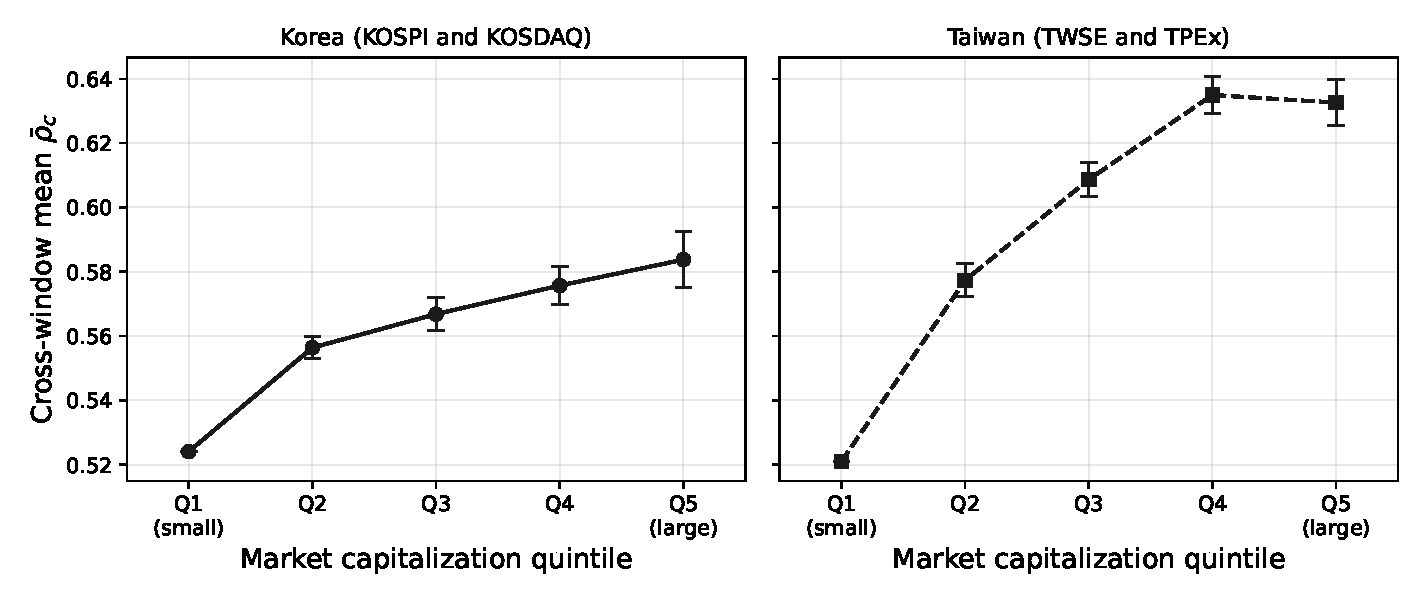
\includegraphics[width=0.92\textwidth]{../figures/fig_headline_gradient.pdf}
\caption{Cross-window mean percolation threshold $\bar\rho_c$ by market-capitalization quintile, Korea (left) and Taiwan (right), on one vertical scale. Quintiles run from Q1 (smallest market capitalization) to Q5 (largest). Each point averages $\rho_c$ over the market's rolling \paperWindowDays-day windows. Error bars are one Newey--West HAC standard error of the mean difference between the quintile's $\rho_c$ and Q1's in the same window, so Q1 has no bar. The means of both markets rise from Q1 through Q4, whereas from Q4 to Q5 Korea's mean rises and Taiwan's falls slightly.}
\label{fig:headline_gradient}
\end{figure}

\begin{table}[pos=htbp]
\centering
\begin{threeparttable}
\caption{Percolation threshold and mean correlation by market-capitalization quintile, Korea. Each median, mean, standard deviation, minimum and maximum is taken over the windows.}\label{tab:percolation}
\begin{tabular}{lccccc}
\toprule
Statistic & Q1 (small) & Q2 & Q3 & Q4 & Q5 (large) \\
\midrule
Number of windows           & \nWindowsHeadline & \nWindowsHeadline & \nWindowsHeadline & \nWindowsHeadline & \nWindowsHeadline \\
Median stocks per window    & \medianStocksHeadlineQone & \medianStocksHeadlineQtwo & \medianStocksHeadlineQthree & \medianStocksHeadlineQfour & \medianStocksHeadlineQfive \\
Mean $\rho_c$               & \barRhoCQone & \barRhoCQtwo & \barRhoCQthree & \barRhoCQfour & \barRhoCQfive \\
Standard deviation of $\rho_c$ & \rhoCStdHeadlineQone & \rhoCStdHeadlineQtwo & \rhoCStdHeadlineQthree & \rhoCStdHeadlineQfour & \rhoCStdHeadlineQfive \\
Minimum $\rho_c$            & \rhoCMinHeadlineQone & \rhoCMinHeadlineQtwo & \rhoCMinHeadlineQthree & \rhoCMinHeadlineQfour & \rhoCMinHeadlineQfive \\
Maximum $\rho_c$            & \rhoCMaxHeadlineQone & \rhoCMaxHeadlineQtwo & \rhoCMaxHeadlineQthree & \rhoCMaxHeadlineQfour & \rhoCMaxHeadlineQfive \\
Mean $\rho_c^{\chi}$        & \barRhoCChiQone & \barRhoCChiQtwo & \barRhoCChiQthree & \barRhoCChiQfour & \barRhoCChiQfive \\
\midrule
Mean $|\rho_{ij}|$          & \meanAbsCorrQone & \meanAbsCorrQtwo & \meanAbsCorrQthree & \meanAbsCorrQfour & \meanAbsCorrQfive \\
\bottomrule
\end{tabular}
\end{threeparttable}
\end{table}

Tests robust to the overlap of the windows find the three steps through Q4 and the endpoint contrast significant and the Q4--Q5 step not (Table~\ref{tab:pair_significance}). The ordering Q1 $<$ Q2 $<$ Q3 $<$ Q4 is therefore significant at the $5\%$ level, whereas the ordering through Q5 is not. In Korea, the tests with both the bandwidth and the block length set to \bwShort\ windows, and with both set to \bwLong\ windows, find the same steps significant (Supplementary Material, Table~\ref{tab:step_robustness}).

\begin{table}[pos=htbp]
\centering
\begin{threeparttable}
\caption{One-sided tests of a rise in $\rho_c$ between adjacent quintiles and between Q1 and Q5, Korea.}\label{tab:pair_significance}
\begin{tabular}{lcc}
\toprule
Pair & HAC $t$ & Block bootstrap $p$ \\
\midrule
Q1--Q2 & $\tHacQoneQtwo$   & $<\pBlockBootQoneQtwo$ \\
Q2--Q3 & $\tHacQtwoQthree$ & $\pBlockBootQtwoQthree$ \\
Q3--Q4 & $\tHacQthreeQfour$ & $\pBlockBootQthreeQfour$ \\
Q4--Q5 & $\tHacQfourQfive$ & $\pBlockBootQfourQfive$ \\
\midrule
Q1--Q5 (endpoint) & $\tHacQoneQfive$ & $<\pBlockBootQoneQfive$ \\
\bottomrule
\end{tabular}
\end{threeparttable}
\end{table}

\paragraph{Noise.} Noise alone, which the shuffled-returns null leaves, reverses the endpoint contrast, whereas removing noise by Marchenko--Pastur clipping widens it (Table~\ref{tab:robustness_contrast}). The shuffled-returns null removes every correlation between stocks and is the only check that reverses the contrast. Marchenko--Pastur clipping replaces the eigenvalues that independent series would produce and keeps the five means ordered.

\paragraph{Estimation settings.} The five means stay ordered at each window length and observation requirement. The endpoint contrast widens with the window length between \windowDaysWthirty\ and \windowDaysWtwofifty\ days, so choosing the \paperWindowDays-day window for the main estimate does not enlarge the contrast. The susceptibility-peak threshold $\rho_c^{\chi}$ rises at every step except Q3--Q4, at which its two means are equal at three decimals and the step is not significant, so its ordering through Q4 is not significant (Table~\ref{tab:percolation}; Supplementary Material, Sec.~\ref{subsec:researcher_choices}).

\paragraph{Stale prices.} Weekly returns reproduce the Korean endpoint contrast but not every Korean step through Q4. $\rho_c$ located in Korean weekly returns on windows of \wkWindowShort\ and \wkWindowLong\ days keeps a significant endpoint contrast at both lengths (Supplementary Material, Table~\ref{tab:weekly_rho_c}). Weekly returns reproduce the Q1--Q2 step at both lengths, the Q2--Q3 step only at \wkWindowLong\ days, and the Q3--Q4 step only at \wkWindowShort\ days. The weekly Q2--Q3 step at \wkWindowShort\ days and the weekly Q3--Q4 step at \wkWindowLong\ days are not significant, although at each of these lengths the weekly test detects a step of the daily step's size with \detectPowerPct\ power, so stale prices could produce either daily step. On the windows of \wkWindowShort\ and \wkWindowLong\ days, the daily Korean Q4--Q5 step is significant, unlike on the \paperWindowDays-day windows of the main estimate. The weekly Q4--Q5 step is not significant at either length, although the weekly test detects a step of the daily step's size with \detectPowerPct\ power, so stale prices could produce the daily step, which therefore does not extend the claim to Q5.

\paragraph{Exchange board and sector mix.} Ranking size within sectors keeps \rhoCGapWithinSectorPctOfHeadline\ of the endpoint contrast and the ordering of all five means, but its Q3--Q4 step is not significant, so its ordering through Q4 is not significant. The KOSPI-only panel keeps a positive endpoint contrast, but neither its Q2--Q3 step nor its Q3--Q4 step, at which its two means reverse, is significant. Its test detects with \detectPowerPct\ power only a step larger than either of these two steps of the main estimate, so the KOSPI-only check neither confirms nor refutes them (Supplementary Material, Sec.~\ref{subsec:size_confounds}).

\begin{table}[pos=htbp]
\centering
\begin{threeparttable}
\caption{Endpoint contrast $\bar\rho_c(\text{Q5}) - \bar\rho_c(\text{Q1})$ under each check, Korea, grouped by the alternative that the check addresses. ``Ordering'' reads ``ordered'' if the five cross-window means rise at every step at three decimals. Otherwise it names the step whose two means reverse or are equal at three decimals, or reads ``reversed'' if the Q5 mean lies below the Q1 mean.}\label{tab:robustness_contrast}
\footnotesize
\begin{tabular}{l c l}
\toprule
Check & Endpoint contrast & Ordering \\
\midrule
\multicolumn{3}{l}{\textit{Noise}} \\
Marchenko--Pastur clipping & $+\rhoCGapRmt$ & ordered \\
Shuffled-returns null & $\shuffNullGapQFiveMinusQone$ & reversed \\
\addlinespace
\multicolumn{3}{l}{\textit{Stale prices}} \\
Weekly threshold, $T = \wkWindowShort$\tnote{a} & $\wkKrShortWeeklyStepQoneQfive$ & Q4--Q5 equal \\
Weekly threshold, $T = \wkWindowLong$\tnote{a} & $\wkKrLongWeeklyStepQoneQfive$ & ordered \\
\addlinespace
\multicolumn{3}{l}{\textit{A variable that moves with size}} \\
KOSPI-only panel & $+\rhoCGapKospi$ & Q3--Q4 reversed \\
Within-sector quintiles & $+\rhoCGapWithinSector$ & ordered \\
\addlinespace
\multicolumn{3}{l}{\textit{Estimation settings}} \\
Window length $T = \windowDaysWthirty$ & $+\rhoCGapWthirty$ & ordered \\
Window length $T = \windowDaysWhundredtwenty$ & $+\rhoCGapWhundredtwenty$ & ordered \\
Window length $T = \windowDaysWtwofifty$ & $+\rhoCGapWtwofifty$ & ordered \\
Observation requirement \minValidFractionLoPct & $+\rhoCGapObsReqLo$ & ordered \\
Observation requirement \minValidFractionHiPct & $+\rhoCGapObsReqHi$ & ordered \\
Susceptibility peak $\rho_c^{\chi}$ & $+\rhoCGapChi$ & Q3--Q4 equal \\
\bottomrule
\end{tabular}
\begin{tablenotes}
\footnotesize
\item[a] Endpoint contrast of $\rho_c$ located in weekly returns on windows of $T$ trading days, and the ordering of its five cross-window means.
\end{tablenotes}
\end{threeparttable}
\end{table}

\paragraph{Common-factor residuals.}\label{subsec:residuals} Removing common-factor returns removes most of the rise from Q1 to Q4 (Table~\ref{tab:residual_steps}). The rise is \rhoCRiseQoneQfourHeadline\ in raw returns and lies between \rhoCRiseQoneQfourResidMin\ and \rhoCRiseQoneQfourResidMax\ in the residuals of each of the four factor constructions. The residual Q4--Q5 step depends on the factor construction, so the residual endpoint contrast, which is the sum of that step and the residual rise from Q1 to Q4, depends on the construction too.

\begin{table}[pos=htbp]
\centering
\begin{threeparttable}
\caption{Adjacent-quintile steps and endpoint contrast of $\bar\rho_c$ in raw returns and in the residuals of the four common-factor constructions, Korea. Each cell gives the step and, in parentheses, its Newey--West HAC $t$-statistic.}\label{tab:residual_steps}
\footnotesize
\setlength{\tabcolsep}{4pt}
\begin{tabular}{l ccccc}
\toprule
Returns & Q1--Q2 & Q2--Q3 & Q3--Q4 & Q4--Q5 & Q1--Q5 \\
\midrule
Raw & $\rhoCStepHeadlineQoneQtwo$ ($\tHacQoneQtwo$) & $\rhoCStepHeadlineQtwoQthree$ ($\tHacQtwoQthree$) & $\rhoCStepHeadlineQthreeQfour$ ($\tHacQthreeQfour$) & $\rhoCStepHeadlineQfourQfive$ ($\tHacQfourQfive$) & $+\rhoCGapHeadline$ ($\tHacQoneQfive$) \\
\addlinespace
\multicolumn{6}{l}{\textit{Residual of}} \\
\quad Market, cap-weighted & $\rhoCStepMktResidQoneQtwo$ ($\tHacMktResidQoneQtwo$) & $\rhoCStepMktResidQtwoQthree$ ($\tHacMktResidQtwoQthree$) & $\rhoCStepMktResidQthreeQfour$ ($\tHacMktResidQthreeQfour$) & $\rhoCStepMktResidQfourQfive$ ($\tHacMktResidQfourQfive$) & $\rhoCGapMktResid$ ($\tHacMktResidQoneQfive$) \\
\quad Market, equal-weighted & $\rhoCStepMktResidEwQoneQtwo$ ($\tHacMktResidEwQoneQtwo$) & $\rhoCStepMktResidEwQtwoQthree$ ($\tHacMktResidEwQtwoQthree$) & $\rhoCStepMktResidEwQthreeQfour$ ($\tHacMktResidEwQthreeQfour$) & $\rhoCStepMktResidEwQfourQfive$ ($\tHacMktResidEwQfourQfive$) & $\rhoCGapMktResidEw$ ($\tHacMktResidEwQoneQfive$) \\
\quad Market $+$ sector, cap-weighted & $\rhoCStepMktSecResidQoneQtwo$ ($\tHacMktSecResidQoneQtwo$) & $\rhoCStepMktSecResidQtwoQthree$ ($\tHacMktSecResidQtwoQthree$) & $\rhoCStepMktSecResidQthreeQfour$ ($\tHacMktSecResidQthreeQfour$) & $\rhoCStepMktSecResidQfourQfive$ ($\tHacMktSecResidQfourQfive$) & $\rhoCGapMktSecResid$ ($\tHacMktSecResidQoneQfive$) \\
\quad Market $+$ sector, equal-weighted & $\rhoCStepMktSecResidEwQoneQtwo$ ($\tHacMktSecResidEwQoneQtwo$) & $\rhoCStepMktSecResidEwQtwoQthree$ ($\tHacMktSecResidEwQtwoQthree$) & $\rhoCStepMktSecResidEwQthreeQfour$ ($\tHacMktSecResidEwQthreeQfour$) & $\rhoCStepMktSecResidEwQfourQfive$ ($\tHacMktSecResidEwQfourQfive$) & $\rhoCGapMktSecResidEw$ ($\tHacMktSecResidEwQoneQfive$) \\
\bottomrule
\end{tabular}
\end{threeparttable}
\end{table}

\paragraph{Subperiods.}\label{subsec:subperiod} The Korean endpoint contrast varies over time, but Q1's threshold lies below Q5's in most windows (Fig.~\ref{fig:rolling_rho_c}). The endpoint contrast in the second half of the windows (the \nWindowsSecondHalf\ windows from \secondHalfStart) is \rhoCGapEndpointLate, \rhoCGapLateShareOfEarlyPct\ of its first-half value of \rhoCGapEndpointEarly. The second-half contrast stays significant (Table~\ref{tab:subperiod}; block bootstrap $p = \pBootEndpointLate$) and is positive in \fracWindowsLateQoneLtQfive\ of the second-half windows. In the second half, the Q1--Q2 step of \rhoCStepSecondHalfQoneQtwo\ is significant (HAC $t = \tHacSecondHalfQoneQtwo$), whereas neither the Q2--Q3 step (HAC $t = \tHacSecondHalfQtwoQthree$) nor the Q3--Q4 step (HAC $t = \tHacSecondHalfQthreeQfour$) is. The means of Q2, Q3, and Q4 lie within \rhoCSecondHalfInteriorSpan\ of each other. In the second half, the Q4--Q5 step is $\rhoCStepSecondHalfQfourQfive$ (HAC $t = \tHacSecondHalfQfourQfive$), so Q5's mean lies below Q4's mean. Among the five-year periods, the endpoint contrast is not significant in \krUnresolvedBlock\ alone.

\begin{figure}[htbp]
\centering
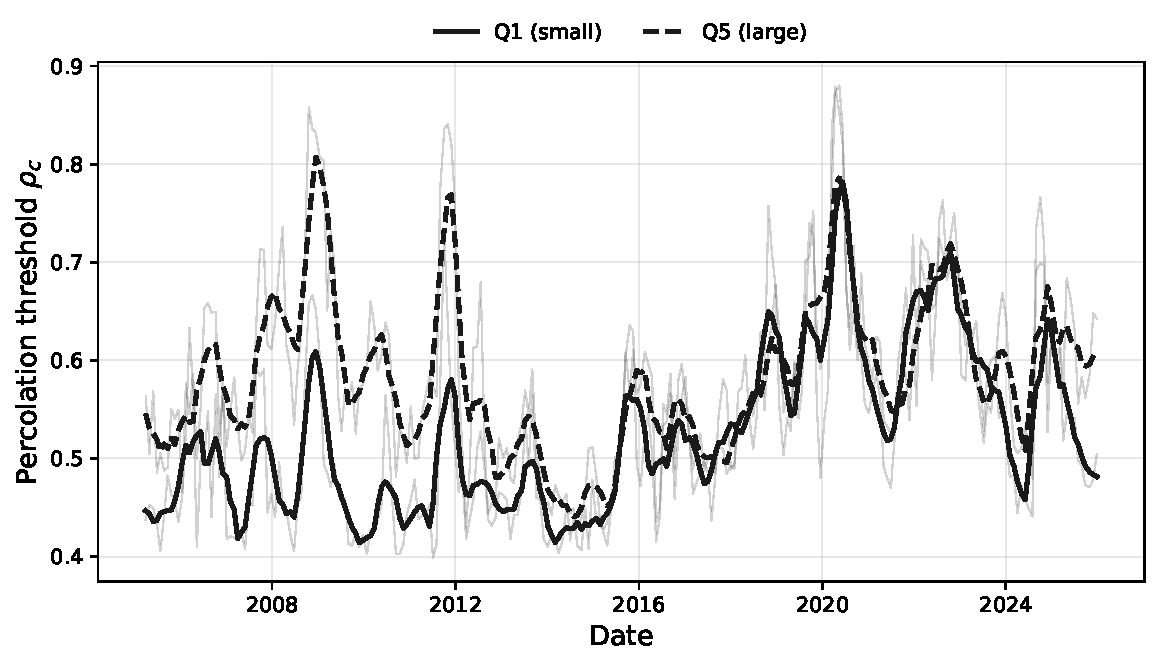
\includegraphics[width=0.85\textwidth]{../figures/fig_rolling_rho_c.pdf}
\caption{Percolation threshold $\rho_c$ of Q1 (smallest market capitalization) and Q5 (largest) in each rolling \paperWindowDays-day window, Korea, \paperSampleStart--\paperSampleEnd. Faint lines are the per-window means over the \nDrawSeeds\ draws, and bold lines are a centered moving average over \rollingMASteps\ windows. The Q5 line lies above the Q1 line in most windows.}
\label{fig:rolling_rho_c}
\end{figure}

\begin{table}[pos=htbp]
\centering
\begin{threeparttable}
\caption{One-sided Newey--West HAC $t$-statistic of the endpoint contrast in each subperiod, Korea and Taiwan.}\label{tab:subperiod}
\begin{tabular}{lcc}
\toprule
Windows & Korea & Taiwan \\
\midrule
All & \tHacQoneQfive & \tHacTwQoneQfive \\
First half  & \tHacEndpointEarly & \tHacEndpointEarlyTw \\
Second half & \tHacEndpointLate  & \tHacEndpointLateTw \\
\addlinespace
\yearBlockA & \tHacYearBlockKrA & \tHacYearBlockTwA \\
\yearBlockB & \tHacYearBlockKrB & \tHacYearBlockTwB \\
\yearBlockC & \tHacYearBlockKrC & \tHacYearBlockTwC \\
\yearBlockD & \tHacYearBlockKrD & \tHacYearBlockTwD \\
\bottomrule
\end{tabular}
\end{threeparttable}
\end{table}

\subsection{Taiwan: the Threshold Rises Significantly Through the Fourth Quintile}\label{subsec:taiwan}

In Taiwan, $\bar\rho_c$ rises from \barRhoCTwQone\ in Q1 to \barRhoCTwQfour\ in Q4 and is \barRhoCTwQfive\ in Q5 (Table~\ref{tab:taiwan_rerun} and Fig.~\ref{fig:headline_gradient}). Each of the three steps through Q4 is significant, with HAC $t$-statistics between \tHacTwQtwoQthree\ and \tHacTwQoneQtwo. The Q4--Q5 step, $\rhoCGapTwQFiveMinusQFour$, is not significant (HAC $t = \tHacTwQfourQfive$). Because the Korean Q4--Q5 step is positive, the two markets differ in the sign of the Q4--Q5 step, although the step is significant in neither market. The Taiwanese endpoint contrast is \rhoCGapTw, with a HAC $t$-statistic of \tHacTwQoneQfive, compared with \tHacQoneQfive\ in Korea. Q1's $\rho_c$ is below Q5's in \fracWindowsQoneLtQfiveTw\ of the Taiwanese windows and in \fracWindowsQoneLtQfiveKr\ of the Korean ones. The susceptibility-peak threshold $\rho_c^{\chi}$ also rises through Q4, and each of its three steps through Q4 is significant, with HAC $t$-statistics between \tHacTwChiStepMin\ and \tHacTwChiStepMax. It falls slightly into Q5, with an endpoint HAC $t$-statistic of \tHacTwChiQoneQfive\ and a Q4--Q5 HAC $t$-statistic of \tHacTwChiQfourQfive. The tests with both the bandwidth and the block length set to \bwShort\ windows, and with both set to \bwLong\ windows, find the same Taiwanese steps significant (Supplementary Material, Table~\ref{tab:step_robustness}). Weekly returns reproduce the Taiwanese endpoint contrast and each Taiwanese step through Q4 on both window lengths of the weekly-threshold check (Supplementary Material, Table~\ref{tab:weekly_rho_c}).

\begin{table}[pos=htbp]
\centering
\begin{threeparttable}
\caption{Percolation threshold by market-capitalization quintile, Taiwan. In the test rows, the column of each quintile tests the step from the previous quintile, and column Q1--Q5 tests the endpoint contrast. Every test is one-sided for a rise.}\label{tab:taiwan_rerun}
\begin{tabular}{lcccccc}
\toprule
Statistic & Q1 (small) & Q2 & Q3 & Q4 & Q5 (large) & Q1--Q5 \\
\midrule
Number of windows           & \nWindowsTw & \nWindowsTw & \nWindowsTw & \nWindowsTw & \nWindowsTw & \\
Median stocks per window    & \medianStocksTwQone & \medianStocksTwQtwo & \medianStocksTwQthree & \medianStocksTwQfour & \medianStocksTwQfive & \\
Mean $\rho_c$               & \barRhoCTwQone & \barRhoCTwQtwo & \barRhoCTwQthree & \barRhoCTwQfour & \barRhoCTwQfive & \\
Mean $\rho_c^{\chi}$        & \barRhoCChiTwQone & \barRhoCChiTwQtwo & \barRhoCChiTwQthree & \barRhoCChiTwQfour & \barRhoCChiTwQfive & \\
\midrule
HAC $t$ & --- & $\tHacTwQoneQtwo$ & $\tHacTwQtwoQthree$ & $\tHacTwQthreeQfour$ & $\tHacTwQfourQfive$ & $\tHacTwQoneQfive$ \\
Block bootstrap $p$ & --- & $<\pBlockBootTwQoneQtwo$ & $<\pBlockBootTwQtwoQthree$ & $<\pBlockBootTwQthreeQfour$ & $\pBlockBootTwQfourQfive$ & $<\pBlockBootTwQoneQfive$ \\
\bottomrule
\end{tabular}
\end{threeparttable}
\end{table}

The Taiwanese endpoint contrast falls from \rhoCGapEndpointEarlyTw\ in the first half of the windows to \rhoCGapEndpointLateTw\ in the second, \rhoCGapLateShareOfEarlyTwPct\ of its first-half value, whereas the Korean endpoint contrast falls to \rhoCGapLateShareOfEarlyPct\ of its first-half value. The Taiwanese HAC $t$-statistic is at least \tHacYearBlockTwA\ in every five-year period (Table~\ref{tab:subperiod}).

\subsection{The Threshold Rises with the Network Size and the Mean Correlation Does Not}\label{subsec:threshold_vs_mean}

Across the quintiles, $\rho_c$ moves with the mean correlation of the same stocks, but the mean correlation does not account for the whole rise in $\rho_c$. Over all Korean (window, quintile) cells, the Spearman rank correlation between $\rho_c$ and the mean $|\rho_{ij}|$ is \meanCorrSpearman. The mean $|\rho_{ij}|$ rises at every step, by only $\meanCorrStepQfourQfive$ from Q4 to Q5 (Table~\ref{tab:percolation}), so it orders the quintiles as $\bar\rho_c$ does. A cubic regression of $\rho_c$ on the mean $|\rho_{ij}|$ over all cells leaves residuals whose quintile means still rise at every step, with an endpoint contrast of \rhoCResidGapPctOfRaw\ of that of $\rho_c$ (Supplementary Material, Sec.~\ref{si:rho_c_vs_mean}). Polynomials of degree one to five leave residuals that rise at every step, with endpoint contrasts between \rhoCResidGapPctOfRawDegLo\ and \rhoCResidGapPctOfRawDegHi\ of that of $\rho_c$.

Across network sizes, $\rho_c$ and the mean correlation diverge, as Eq.~\eqref{eq:toy_closed_form} predicts, so $\rho_c$ is not a function of the mean correlation alone. In the regression on $\sqrt{2\ln(N-1)}$, the pooled slope of $\rho_c$ is \rhoCSlopeSqrtLogN\ ($R^2 = \rhoCSlopeSqrtLogNRsq$) and is positive in every quintile, whereas the pooled slope of the mean $|\rho_{ij}|$ is \meanCorrSlopeSqrtLogN\ to three decimal places. From $N = \networkSizeNMin$ to \networkSizeNMax, $\rho_c$ rises by \dgpNScalingDriftEmpiricalLo\ to \dgpNScalingDriftEmpiricalHi\ across the quintiles, whereas the mean $|\rho_{ij}|$ changes by only \meanCorrDriftFiftyToThreeHundredLo\ to \meanCorrDriftFiftyToThreeHundredHi. Because Q1 holds fewer stocks than Q5 in each window, the network size alone produces part of the endpoint contrast. Applied to the network sizes of Q1 and Q5 in each window, the Korean pooled slope accounts for \rhoCGapKrNImplied\ (\rhoCGapKrNImpliedPct) of the Korean endpoint contrast and for \rhoCGapTwNImplied\ (\rhoCGapTwNImpliedPct) of the Taiwanese one.

% ============================================================
% 5. DISCUSSION
% ============================================================
\section{Discussion}\label{sec:discussion}

\subsection{What the Rise Identifies}\label{subsec:dissipation_mechanism}

None of the exchange board, the sector mix, and the estimation settings accounts for the endpoint contrast, whereas stale prices could account for the Korean Q2--Q3 and Q3--Q4 steps. The shuffled-returns null leaves only noise and reverses the endpoint contrast, because Q1's returns have the heaviest tails, which widen the sampling distribution of the correlations of independent series and so raise its upper quantile, where $\rho_c$ lies (Supplementary Material, Sec.~\ref{subsec:null_robustness}). Marchenko--Pastur clipping widens the endpoint contrast, so the rise lies in the eigenvalues outside the band $[\lambda_-, \lambda_+]$.

Each of two further sources, lower loadings of small caps on common factors and weaker propagation among them, would produce the rise from Q1 to Q4 that the residuals from regressions on market and sector returns remove. The residuals therefore cannot distinguish the two sources (Section~\ref{subsec:toy_model}). The two sources could be separated by testing whether pairs of stocks that index funds and ETFs hold in common are more correlated than their factor loadings imply.

The largest sample correlation grows with the number of variables both in independent populations (Section~\ref{subsec:network_size}) and in equi-correlated ones, in which every pair has the same correlation~\citep{fan2019largest}. $\rho_c$ lies in the upper tail of the sample correlations, so its rise with the network size would appear whatever produces the correlations. The divergence of $\rho_c$ from the mean correlation across network sizes, which Eq.~\eqref{eq:toy_closed_form} predicts, therefore does not test the model. \citet{shirazi2017noncriticality} found the threshold of their network of S\&P~500 stocks independent of network size, which does not conflict with the rise of $\rho_c$, because their network links stocks by partial correlations rather than by raw correlations.

\subsection{Scope of the Claim}\label{subsec:limits}

The estimation limits the claim in four ways, which concern the stocks that each window holds, stale prices, the Korean Q3--Q4 step, and the window length. The quintiles hold the stocks listed at each window's end, and the observation requirement drops each stock whose share of non-missing daily returns in the window does not exceed \minValidFractionPct, so each window's $\rho_c$ describes the stocks that survived the window and traded on most of its days. The Taiwanese quintiles, which lack the delisted stocks that FinMind does not price, are not free of survivorship bias. The weekly-threshold check uses windows of \wkWindowShort\ and \wkWindowLong\ days, so the part of the endpoint contrast that stale prices produce on the \paperWindowDays-day windows of the main estimate is not bounded. The Korean Q3--Q4 step, which is not significant when size is ranked within sectors or when the threshold is located by the susceptibility peak, depends on how size and the threshold are measured. The claim concerns the direction of the rise at a fixed window length and not the level of $\rho_c$, which falls as the window lengthens (Supplementary Material, Sec.~\ref{subsec:researcher_choices}).

The sample limits the claim in two further ways. The Korean rise through Q4 holds for all windows taken together rather than for every period. Korea and Taiwan lie in one region, so the Taiwanese panel does not test the rise under the macroeconomic conditions of another region.

% ============================================================
% 6. CONCLUSION
% ============================================================
\section{Conclusion}\label{sec:conclusion}

Studies of threshold-correlation graphs estimate at most one percolation threshold $\rho_c$ per market, so the variation of $\rho_c$ across the size segments of one market has been unmeasured. We estimated $\rho_c$ in each size quintile of the Korean and Taiwanese stock markets and predicted its cross-quintile ordering with a return-generating model in which the weight of each stock's own shocks in its return falls with firm size. Over all windows of \paperSampleStart--\paperSampleEnd\ taken together, the mean $\rho_c$ of raw returns rises with firm size significantly through the fourth quintile in both markets. The model predicts this rise with no parameter calibrated to data if that weight, the factor loadings, and the propagation of shocks between stocks meet the conditions of Section~\ref{subsec:toy_model}. The model also predicts a rise from the fourth to the largest quintile, whereas that step is not significant in Korea and is slightly negative in Taiwan. Weekly returns reproduce each Taiwanese step through the fourth quintile, but in Korea they reproduce at both window lengths only the step from the smallest quintile and the endpoint contrast. In Korea, unlike the mean correlation of the same stocks, $\rho_c$ rises with the number of stocks drawn per quintile, so $\rho_c$ is not a function of the mean correlation alone. In Korea, most of the rise to the fourth quintile disappears in the residuals from regressions on market and sector returns. Because $\rho_c$ rises with firm size through the fourth quintile, a difference in $\rho_c$ between two markets or two periods can reflect their mix of firm sizes rather than how strongly stocks of one size are correlated.

% ============================================================
% DECLARATIONS
% ============================================================
\section*{CRediT authorship contribution statement}

\noindent \textbf{Sungwoo Kang:} Conceptualization, Methodology, Software, Formal analysis, Data curation, Writing -- original draft, Writing -- review \& editing, Visualization. \textbf{Jong-Kook Kim:} Writing -- review \& editing.

\section*{Declaration of competing interest}

\noindent The authors declare that they have no known competing financial interests or personal relationships that could have appeared to influence the work reported in this paper.

\section*{Data availability}

\noindent The Korean adjusted closes come from the proprietary FnGuide DataGuide service and cannot be redistributed. The open-source \texttt{marcap} dataset supplies the Korean stocks listed on each day and their market capitalizations. The Korea Exchange supplies the Korean sector classification. The Taiwanese data are derived from the open-source FinMind dataset. The analysis code and the processed outputs that reproduce every table and figure are available at \url{https://github.com/hpicsk/percolation}. Only the two scripts that build the Korean and Taiwanese panels read the FnGuide and FinMind data. The repository holds the daily returns and market capitalizations that those scripts compute, but not the FnGuide adjusted closes.

\section*{Declaration of generative AI and AI-assisted technologies in the manuscript preparation process}

\noindent The authors used Claude (Anthropic) to assist with code implementation as well as to improve the readability and language of the manuscript. The authors reviewed and edited the content as needed and take full responsibility for the content of the publication.

\section*{Acknowledgments}

\noindent This research did not receive any specific grant from funding agencies in the public, commercial, or not-for-profit sectors.

% ============================================================
% REFERENCES
% ============================================================
\bibliographystyle{elsarticle-num-names}
\bibliography{references}

\end{document}
